\documentclass[twoside]{book}

% Packages required by doxygen
\usepackage{fixltx2e}
\usepackage{calc}
\usepackage{doxygen}
\usepackage[export]{adjustbox} % also loads graphicx
\usepackage{graphicx}
\usepackage[utf8]{inputenc}
\usepackage{makeidx}
\usepackage{multicol}
\usepackage{multirow}
\PassOptionsToPackage{warn}{textcomp}
\usepackage{textcomp}
\usepackage[nointegrals]{wasysym}
\usepackage[table]{xcolor}

% Font selection
\usepackage[T1]{fontenc}
\usepackage[scaled=.90]{helvet}
\usepackage{courier}
\usepackage{amssymb}
\usepackage{sectsty}
\renewcommand{\familydefault}{\sfdefault}
\allsectionsfont{%
  \fontseries{bc}\selectfont%
  \color{darkgray}%
}
\renewcommand{\DoxyLabelFont}{%
  \fontseries{bc}\selectfont%
  \color{darkgray}%
}
\newcommand{\+}{\discretionary{\mbox{\scriptsize$\hookleftarrow$}}{}{}}

% Page & text layout
\usepackage{geometry}
\geometry{%
  a4paper,%
  top=2.5cm,%
  bottom=2.5cm,%
  left=2.5cm,%
  right=2.5cm%
}
\tolerance=750
\hfuzz=15pt
\hbadness=750
\setlength{\emergencystretch}{15pt}
\setlength{\parindent}{0cm}
\setlength{\parskip}{3ex plus 2ex minus 2ex}
\makeatletter
\renewcommand{\paragraph}{%
  \@startsection{paragraph}{4}{0ex}{-1.0ex}{1.0ex}{%
    \normalfont\normalsize\bfseries\SS@parafont%
  }%
}
\renewcommand{\subparagraph}{%
  \@startsection{subparagraph}{5}{0ex}{-1.0ex}{1.0ex}{%
    \normalfont\normalsize\bfseries\SS@subparafont%
  }%
}
\makeatother

% Headers & footers
\usepackage{fancyhdr}
\pagestyle{fancyplain}
\fancyhead[LE]{\fancyplain{}{\bfseries\thepage}}
\fancyhead[CE]{\fancyplain{}{}}
\fancyhead[RE]{\fancyplain{}{\bfseries\leftmark}}
\fancyhead[LO]{\fancyplain{}{\bfseries\rightmark}}
\fancyhead[CO]{\fancyplain{}{}}
\fancyhead[RO]{\fancyplain{}{\bfseries\thepage}}
\fancyfoot[LE]{\fancyplain{}{}}
\fancyfoot[CE]{\fancyplain{}{}}
\fancyfoot[RE]{\fancyplain{}{\bfseries\scriptsize Generated by Doxygen }}
\fancyfoot[LO]{\fancyplain{}{\bfseries\scriptsize Generated by Doxygen }}
\fancyfoot[CO]{\fancyplain{}{}}
\fancyfoot[RO]{\fancyplain{}{}}
\renewcommand{\footrulewidth}{0.4pt}
\renewcommand{\chaptermark}[1]{%
  \markboth{#1}{}%
}
\renewcommand{\sectionmark}[1]{%
  \markright{\thesection\ #1}%
}

% Indices & bibliography
\usepackage{natbib}
\usepackage[titles]{tocloft}
\setcounter{tocdepth}{3}
\setcounter{secnumdepth}{5}
\makeindex

% Hyperlinks (required, but should be loaded last)
\usepackage{ifpdf}
\ifpdf
  \usepackage[pdftex,pagebackref=true]{hyperref}
\else
  \usepackage[ps2pdf,pagebackref=true]{hyperref}
\fi
\hypersetup{%
  colorlinks=true,%
  linkcolor=blue,%
  citecolor=blue,%
  unicode%
}

% Custom commands
\newcommand{\clearemptydoublepage}{%
  \newpage{\pagestyle{empty}\cleardoublepage}%
}

\usepackage{caption}
\captionsetup{labelsep=space,justification=centering,font={bf},singlelinecheck=off,skip=4pt,position=top}

%===== C O N T E N T S =====

\begin{document}

% Titlepage & ToC
\hypersetup{pageanchor=false,
             bookmarksnumbered=true,
             pdfencoding=unicode
            }
\pagenumbering{alph}
\begin{titlepage}
\vspace*{7cm}
\begin{center}%
{\Large LA meets ML }\\
\vspace*{1cm}
{\large Generated by Doxygen 1.8.14}\\
\end{center}
\end{titlepage}
\clearemptydoublepage
\pagenumbering{roman}
\tableofcontents
\clearemptydoublepage
\pagenumbering{arabic}
\hypersetup{pageanchor=true}

%--- Begin generated contents ---
\chapter{Hierarchical Index}
\section{Class Hierarchy}
This inheritance list is sorted roughly, but not completely, alphabetically\+:\begin{DoxyCompactList}
\item \contentsline{section}{modules.\+model.\+classification\+\_\+module.\+classification\+\_\+module.\+Classifier}{\pageref{classmodules_1_1model_1_1classification__module_1_1classification__module_1_1_classifier}}{}
\item \contentsline{section}{modules.\+model.\+collector\+\_\+module.\+collector.\+Collector}{\pageref{classmodules_1_1model_1_1collector__module_1_1collector_1_1_collector}}{}
\item \contentsline{section}{modules.\+controller.\+commands.\+command.\+Command}{\pageref{classmodules_1_1controller_1_1commands_1_1command_1_1_command}}{}
\begin{DoxyCompactList}
\item \contentsline{section}{modules.\+controller.\+commands.\+classify\+\_\+command.\+Classify\+Command}{\pageref{classmodules_1_1controller_1_1commands_1_1classify__command_1_1_classify_command}}{}
\item \contentsline{section}{modules.\+controller.\+commands.\+collect\+\_\+command.\+Collect\+Command}{\pageref{classmodules_1_1controller_1_1commands_1_1collect__command_1_1_collect_command}}{}
\item \contentsline{section}{modules.\+controller.\+commands.\+label\+\_\+command.\+Label\+Command}{\pageref{classmodules_1_1controller_1_1commands_1_1label__command_1_1_label_command}}{}
\item \contentsline{section}{modules.\+controller.\+commands.\+quit\+\_\+command.\+Quit\+Command}{\pageref{classmodules_1_1controller_1_1commands_1_1quit__command_1_1_quit_command}}{}
\item \contentsline{section}{modules.\+controller.\+commands.\+train\+\_\+command.\+Train\+Command}{\pageref{classmodules_1_1controller_1_1commands_1_1train__command_1_1_train_command}}{}
\end{DoxyCompactList}
\item \contentsline{section}{modules.\+view.\+command\+\_\+line\+\_\+interface.\+Command\+Line\+Interface}{\pageref{classmodules_1_1view_1_1command__line__interface_1_1_command_line_interface}}{}
\item \contentsline{section}{modules.\+controller.\+command\+\_\+parser.\+Command\+Parser}{\pageref{classmodules_1_1controller_1_1command__parser_1_1_command_parser}}{}
\item \contentsline{section}{modules.\+shared.\+configurations.\+Configurations}{\pageref{classmodules_1_1shared_1_1configurations_1_1_configurations}}{}
\item \contentsline{section}{modules.\+controller.\+controller.\+Controller}{\pageref{classmodules_1_1controller_1_1controller_1_1_controller}}{}
\item Exception\begin{DoxyCompactList}
\item \contentsline{section}{modules.\+exception.\+excpetions.\+My\+Exception}{\pageref{classmodules_1_1exception_1_1excpetions_1_1_my_exception}}{}
\begin{DoxyCompactList}
\item \contentsline{section}{modules.\+exception.\+excpetions.\+Illegal\+Argument\+Exception}{\pageref{classmodules_1_1exception_1_1excpetions_1_1_illegal_argument_exception}}{}
\item \contentsline{section}{modules.\+exception.\+excpetions.\+Invalid\+Config\+Exception}{\pageref{classmodules_1_1exception_1_1excpetions_1_1_invalid_config_exception}}{}
\item \contentsline{section}{modules.\+exception.\+excpetions.\+Invalid\+O\+S\+Exception}{\pageref{classmodules_1_1exception_1_1excpetions_1_1_invalid_o_s_exception}}{}
\item \contentsline{section}{modules.\+exception.\+excpetions.\+I\+O\+Exception}{\pageref{classmodules_1_1exception_1_1excpetions_1_1_i_o_exception}}{}
\end{DoxyCompactList}
\end{DoxyCompactList}
\item \contentsline{section}{modules.\+model.\+collector\+\_\+module.\+generator.\+Generator}{\pageref{classmodules_1_1model_1_1collector__module_1_1generator_1_1_generator}}{}
\item \contentsline{section}{modules.\+model.\+labeling\+\_\+module.\+labeling\+\_\+module.\+Labeling\+Module}{\pageref{classmodules_1_1model_1_1labeling__module_1_1labeling__module_1_1_labeling_module}}{}
\item \contentsline{section}{modules.\+shared.\+loader.\+Loader}{\pageref{classmodules_1_1shared_1_1loader_1_1_loader}}{}
\item \contentsline{section}{modules.\+shared.\+matrix.\+Matrix}{\pageref{classmodules_1_1shared_1_1matrix_1_1_matrix}}{}
\item \contentsline{section}{modules.\+view.\+observable.\+Observable}{\pageref{classmodules_1_1view_1_1observable_1_1_observable}}{}
\item \contentsline{section}{modules.\+view.\+output\+\_\+service.\+Output\+Service}{\pageref{classmodules_1_1view_1_1output__service_1_1_output_service}}{}
\begin{DoxyCompactList}
\item \contentsline{section}{modules.\+view.\+cli\+\_\+output\+\_\+service.\+C\+L\+I\+Output\+Service}{\pageref{classmodules_1_1view_1_1cli__output__service_1_1_c_l_i_output_service}}{}
\end{DoxyCompactList}
\item \contentsline{section}{modules.\+model.\+labeling\+\_\+module.\+preconditioner.\+Preconditioner}{\pageref{classmodules_1_1model_1_1labeling__module_1_1preconditioner_1_1_preconditioner}}{}
\item \contentsline{section}{modules.\+shared.\+saver.\+Saver}{\pageref{classmodules_1_1shared_1_1saver_1_1_saver}}{}
\item \contentsline{section}{modules.\+model.\+labeling\+\_\+module.\+solver.\+Solver}{\pageref{classmodules_1_1model_1_1labeling__module_1_1solver_1_1_solver}}{}
\item \contentsline{section}{modules.\+model.\+collector\+\_\+module.\+ssget.\+S\+S\+Get}{\pageref{classmodules_1_1model_1_1collector__module_1_1ssget_1_1_s_s_get}}{}
\item \contentsline{section}{modules.\+view.\+subscriber.\+Subscriber}{\pageref{classmodules_1_1view_1_1subscriber_1_1_subscriber}}{}
\begin{DoxyCompactList}
\item \contentsline{section}{modules.\+view.\+cli\+\_\+output\+\_\+service.\+C\+L\+I\+Output\+Service}{\pageref{classmodules_1_1view_1_1cli__output__service_1_1_c_l_i_output_service}}{}
\end{DoxyCompactList}
\item \contentsline{section}{modules.\+model.\+training\+\_\+module.\+training\+\_\+module.\+Training\+Module}{\pageref{classmodules_1_1model_1_1training__module_1_1training__module_1_1_training_module}}{}
\item \contentsline{section}{modules.\+shared.\+validator.\+Validator}{\pageref{classmodules_1_1shared_1_1validator_1_1_validator}}{}
\item Enum\begin{DoxyCompactList}
\item \contentsline{section}{modules.\+controller.\+commands.\+key.\+Key}{\pageref{classmodules_1_1controller_1_1commands_1_1key_1_1_key}}{}
\item \contentsline{section}{modules.\+controller.\+commands.\+label\+\_\+mode.\+Label\+Mode}{\pageref{classmodules_1_1controller_1_1commands_1_1label__mode_1_1_label_mode}}{}
\end{DoxyCompactList}
\end{DoxyCompactList}

\chapter{Class Index}
\section{Class List}
Here are the classes, structs, unions and interfaces with brief descriptions\+:\begin{DoxyCompactList}
\item\contentsline{section}{\mbox{\hyperlink{classmodules_1_1model_1_1classification__module_1_1classification__module_1_1_classifier}{modules.\+model.\+classification\+\_\+module.\+classification\+\_\+module.\+Classifier}} \\*This class handles the classification of matrices using a neural network }{\pageref{classmodules_1_1model_1_1classification__module_1_1classification__module_1_1_classifier}}{}
\item\contentsline{section}{\mbox{\hyperlink{classmodules_1_1controller_1_1commands_1_1classify__command_1_1_classify_command}{modules.\+controller.\+commands.\+classify\+\_\+command.\+Classify\+Command}} }{\pageref{classmodules_1_1controller_1_1commands_1_1classify__command_1_1_classify_command}}{}
\item\contentsline{section}{\mbox{\hyperlink{classmodules_1_1view_1_1cli__output__service_1_1_c_l_i_output_service}{modules.\+view.\+cli\+\_\+output\+\_\+service.\+C\+L\+I\+Output\+Service}} \\*This class communicates with the command line interface }{\pageref{classmodules_1_1view_1_1cli__output__service_1_1_c_l_i_output_service}}{}
\item\contentsline{section}{\mbox{\hyperlink{classmodules_1_1controller_1_1commands_1_1collect__command_1_1_collect_command}{modules.\+controller.\+commands.\+collect\+\_\+command.\+Collect\+Command}} }{\pageref{classmodules_1_1controller_1_1commands_1_1collect__command_1_1_collect_command}}{}
\item\contentsline{section}{\mbox{\hyperlink{classmodules_1_1model_1_1collector__module_1_1collector_1_1_collector}{modules.\+model.\+collector\+\_\+module.\+collector.\+Collector}} \\*This class handles the collecting of matrices for further use }{\pageref{classmodules_1_1model_1_1collector__module_1_1collector_1_1_collector}}{}
\item\contentsline{section}{\mbox{\hyperlink{classmodules_1_1controller_1_1commands_1_1command_1_1_command}{modules.\+controller.\+commands.\+command.\+Command}} \\*Interface for the module specific commands }{\pageref{classmodules_1_1controller_1_1commands_1_1command_1_1_command}}{}
\item\contentsline{section}{\mbox{\hyperlink{classmodules_1_1view_1_1command__line__interface_1_1_command_line_interface}{modules.\+view.\+command\+\_\+line\+\_\+interface.\+Command\+Line\+Interface}} \\*Communicates with the command line }{\pageref{classmodules_1_1view_1_1command__line__interface_1_1_command_line_interface}}{}
\item\contentsline{section}{\mbox{\hyperlink{classmodules_1_1controller_1_1command__parser_1_1_command_parser}{modules.\+controller.\+command\+\_\+parser.\+Command\+Parser}} \\*Class for parsing strings to a command }{\pageref{classmodules_1_1controller_1_1command__parser_1_1_command_parser}}{}
\item\contentsline{section}{\mbox{\hyperlink{classmodules_1_1controller_1_1controller_1_1_controller}{modules.\+controller.\+controller.\+Controller}} }{\pageref{classmodules_1_1controller_1_1controller_1_1_controller}}{}
\item\contentsline{section}{\mbox{\hyperlink{classmodules_1_1model_1_1collector__module_1_1generator_1_1_generator}{modules.\+model.\+collector\+\_\+module.\+generator.\+Generator}} \\*This class artificially creates matrices of certain size and denisty }{\pageref{classmodules_1_1model_1_1collector__module_1_1generator_1_1_generator}}{}
\item\contentsline{section}{\mbox{\hyperlink{classmodules_1_1exception_1_1excpetions_1_1_illegal_argument_exception}{modules.\+exception.\+excpetions.\+Illegal\+Argument\+Exception}} }{\pageref{classmodules_1_1exception_1_1excpetions_1_1_illegal_argument_exception}}{}
\item\contentsline{section}{\mbox{\hyperlink{classmodules_1_1exception_1_1excpetions_1_1_invalid_config_exception}{modules.\+exception.\+excpetions.\+Invalid\+Config\+Exception}} }{\pageref{classmodules_1_1exception_1_1excpetions_1_1_invalid_config_exception}}{}
\item\contentsline{section}{\mbox{\hyperlink{classmodules_1_1exception_1_1excpetions_1_1_invalid_o_s_exception}{modules.\+exception.\+excpetions.\+Invalid\+O\+S\+Exception}} }{\pageref{classmodules_1_1exception_1_1excpetions_1_1_invalid_o_s_exception}}{}
\item\contentsline{section}{\mbox{\hyperlink{classmodules_1_1exception_1_1excpetions_1_1_i_o_exception}{modules.\+exception.\+excpetions.\+I\+O\+Exception}} }{\pageref{classmodules_1_1exception_1_1excpetions_1_1_i_o_exception}}{}
\item\contentsline{section}{\mbox{\hyperlink{classmodules_1_1controller_1_1commands_1_1key_1_1_key}{modules.\+controller.\+commands.\+key.\+Key}} }{\pageref{classmodules_1_1controller_1_1commands_1_1key_1_1_key}}{}
\item\contentsline{section}{\mbox{\hyperlink{classmodules_1_1controller_1_1commands_1_1label__command_1_1_label_command}{modules.\+controller.\+commands.\+label\+\_\+command.\+Label\+Command}} }{\pageref{classmodules_1_1controller_1_1commands_1_1label__command_1_1_label_command}}{}
\item\contentsline{section}{\mbox{\hyperlink{classmodules_1_1model_1_1labeling__module_1_1labeling__module_1_1_labeling_module}{modules.\+model.\+labeling\+\_\+module.\+labeling\+\_\+module.\+Labeling\+Module}} \\*This class handles the labeling of the matrices }{\pageref{classmodules_1_1model_1_1labeling__module_1_1labeling__module_1_1_labeling_module}}{}
\item\contentsline{section}{\mbox{\hyperlink{classmodules_1_1controller_1_1commands_1_1label__mode_1_1_label_mode}{modules.\+controller.\+commands.\+label\+\_\+mode.\+Label\+Mode}} }{\pageref{classmodules_1_1controller_1_1commands_1_1label__mode_1_1_label_mode}}{}
\item\contentsline{section}{\mbox{\hyperlink{classmodules_1_1shared_1_1loader_1_1_loader}{modules.\+shared.\+loader.\+Loader}} \\*Class that handles the loading of matrices }{\pageref{classmodules_1_1shared_1_1loader_1_1_loader}}{}
\item\contentsline{section}{\mbox{\hyperlink{classmodules_1_1shared_1_1matrix_1_1_matrix}{modules.\+shared.\+matrix.\+Matrix}} \\*This class represents a matrix holding its values and size }{\pageref{classmodules_1_1shared_1_1matrix_1_1_matrix}}{}
\item\contentsline{section}{\mbox{\hyperlink{classmodules_1_1exception_1_1excpetions_1_1_my_exception}{modules.\+exception.\+excpetions.\+My\+Exception}} }{\pageref{classmodules_1_1exception_1_1excpetions_1_1_my_exception}}{}
\item\contentsline{section}{\mbox{\hyperlink{classmodules_1_1view_1_1observable_1_1_observable}{modules.\+view.\+observable.\+Observable}} \\*Class for creating updating strings }{\pageref{classmodules_1_1view_1_1observable_1_1_observable}}{}
\item\contentsline{section}{\mbox{\hyperlink{classmodules_1_1view_1_1output__service_1_1_output_service}{modules.\+view.\+output\+\_\+service.\+Output\+Service}} \\*Interface for services that can be registered to a module }{\pageref{classmodules_1_1view_1_1output__service_1_1_output_service}}{}
\item\contentsline{section}{\mbox{\hyperlink{classmodules_1_1model_1_1labeling__module_1_1preconditioner_1_1_preconditioner}{modules.\+model.\+labeling\+\_\+module.\+preconditioner.\+Preconditioner}} \\*Abstract class that represents the preconditioners which can be applied to a matrix to fasten the solving process }{\pageref{classmodules_1_1model_1_1labeling__module_1_1preconditioner_1_1_preconditioner}}{}
\item\contentsline{section}{\mbox{\hyperlink{classmodules_1_1controller_1_1commands_1_1quit__command_1_1_quit_command}{modules.\+controller.\+commands.\+quit\+\_\+command.\+Quit\+Command}} }{\pageref{classmodules_1_1controller_1_1commands_1_1quit__command_1_1_quit_command}}{}
\item\contentsline{section}{\mbox{\hyperlink{classmodules_1_1shared_1_1saver_1_1_saver}{modules.\+shared.\+saver.\+Saver}} \\*Class that handles the saving of datasets }{\pageref{classmodules_1_1shared_1_1saver_1_1_saver}}{}
\item\contentsline{section}{\mbox{\hyperlink{classmodules_1_1model_1_1labeling__module_1_1solver_1_1_solver}{modules.\+model.\+labeling\+\_\+module.\+solver.\+Solver}} \\*Abstract class representing the various solvers tht can be executed on the matrices }{\pageref{classmodules_1_1model_1_1labeling__module_1_1solver_1_1_solver}}{}
\item\contentsline{section}{\mbox{\hyperlink{classmodules_1_1model_1_1collector__module_1_1ssget_1_1_s_s_get}{modules.\+model.\+collector\+\_\+module.\+ssget.\+S\+S\+Get}} \\*This class handles the communication with the suit sparse matrix collection using the ssget tool }{\pageref{classmodules_1_1model_1_1collector__module_1_1ssget_1_1_s_s_get}}{}
\item\contentsline{section}{\mbox{\hyperlink{classmodules_1_1view_1_1subscriber_1_1_subscriber}{modules.\+view.\+subscriber.\+Subscriber}} \\*Class than can be registered to an observable }{\pageref{classmodules_1_1view_1_1subscriber_1_1_subscriber}}{}
\item\contentsline{section}{\mbox{\hyperlink{classmodules_1_1controller_1_1commands_1_1train__command_1_1_train_command}{modules.\+controller.\+commands.\+train\+\_\+command.\+Train\+Command}} }{\pageref{classmodules_1_1controller_1_1commands_1_1train__command_1_1_train_command}}{}
\item\contentsline{section}{\mbox{\hyperlink{classmodules_1_1model_1_1training__module_1_1training__module_1_1_training_module}{modules.\+model.\+training\+\_\+module.\+training\+\_\+module.\+Training\+Module}} \\*This class handles the training of the neural network }{\pageref{classmodules_1_1model_1_1training__module_1_1training__module_1_1_training_module}}{}
\item\contentsline{section}{\mbox{\hyperlink{classmodules_1_1shared_1_1validator_1_1_validator}{modules.\+shared.\+validator.\+Validator}} }{\pageref{classmodules_1_1shared_1_1validator_1_1_validator}}{}
\end{DoxyCompactList}

\chapter{Class Documentation}
\hypertarget{classmodules_1_1model_1_1classification__module_1_1classification__module_1_1_classifier}{}\section{modules.\+model.\+classification\+\_\+module.\+classification\+\_\+module.\+Classifier Class Reference}
\label{classmodules_1_1model_1_1classification__module_1_1classification__module_1_1_classifier}\index{modules.\+model.\+classification\+\_\+module.\+classification\+\_\+module.\+Classifier@{modules.\+model.\+classification\+\_\+module.\+classification\+\_\+module.\+Classifier}}


This class handles the classification of matrices using a neural network.  


\subsection*{Static Public Member Functions}
\begin{DoxyCompactItemize}
\item 
def \mbox{\hyperlink{classmodules_1_1model_1_1classification__module_1_1classification__module_1_1_classifier_a0171fa6530689c47b0bfda8bdadd986a}{start}}
\begin{DoxyCompactList}\small\item\em Starts the classification process. \end{DoxyCompactList}\end{DoxyCompactItemize}
\subsection*{Static Public Attributes}
\begin{DoxyCompactItemize}
\item 
\mbox{\Hypertarget{classmodules_1_1model_1_1classification__module_1_1classification__module_1_1_classifier_ae356d5f32bfe960c491f7141d67a5899}\label{classmodules_1_1model_1_1classification__module_1_1classification__module_1_1_classifier_ae356d5f32bfe960c491f7141d67a5899}} 
{\bfseries str}
\end{DoxyCompactItemize}


\subsection{Detailed Description}
This class handles the classification of matrices using a neural network. 

\subsection{Member Function Documentation}
\mbox{\Hypertarget{classmodules_1_1model_1_1classification__module_1_1classification__module_1_1_classifier_a0171fa6530689c47b0bfda8bdadd986a}\label{classmodules_1_1model_1_1classification__module_1_1classification__module_1_1_classifier_a0171fa6530689c47b0bfda8bdadd986a}} 
\index{modules\+::model\+::classification\+\_\+module\+::classification\+\_\+module\+::\+Classifier@{modules\+::model\+::classification\+\_\+module\+::classification\+\_\+module\+::\+Classifier}!start@{start}}
\index{start@{start}!modules\+::model\+::classification\+\_\+module\+::classification\+\_\+module\+::\+Classifier@{modules\+::model\+::classification\+\_\+module\+::classification\+\_\+module\+::\+Classifier}}
\subsubsection{\texorpdfstring{start()}{start()}}
{\footnotesize\ttfamily def modules.\+model.\+classification\+\_\+module.\+classification\+\_\+module.\+Classifier.\+start (\begin{DoxyParamCaption}\item[{}]{path }\end{DoxyParamCaption})\hspace{0.3cm}{\ttfamily [static]}}



Starts the classification process. 


\begin{DoxyParams}{Parameters}
{\em path} & where the matrix that will be classified is located \\
\hline
{\em network} & path where the neural network is located \\
\hline
\end{DoxyParams}


The documentation for this class was generated from the following file\+:\begin{DoxyCompactItemize}
\item 
model/classification\+\_\+module/classification\+\_\+module.\+py\end{DoxyCompactItemize}

\hypertarget{classmodules_1_1controller_1_1commands_1_1classify__command_1_1_classify_command}{}\section{modules.\+controller.\+commands.\+classify\+\_\+command.\+Classify\+Command Class Reference}
\label{classmodules_1_1controller_1_1commands_1_1classify__command_1_1_classify_command}\index{modules.\+controller.\+commands.\+classify\+\_\+command.\+Classify\+Command@{modules.\+controller.\+commands.\+classify\+\_\+command.\+Classify\+Command}}
Inheritance diagram for modules.\+controller.\+commands.\+classify\+\_\+command.\+Classify\+Command\+:\begin{figure}[H]
\begin{center}
\leavevmode
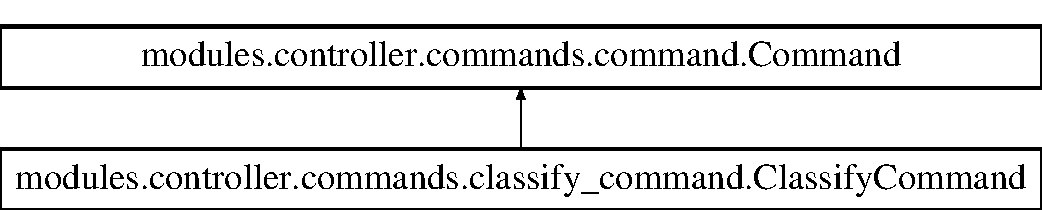
\includegraphics[height=2.000000cm]{classmodules_1_1controller_1_1commands_1_1classify__command_1_1_classify_command}
\end{center}
\end{figure}
\subsection*{Public Member Functions}
\begin{DoxyCompactItemize}
\item 
\mbox{\Hypertarget{classmodules_1_1controller_1_1commands_1_1classify__command_1_1_classify_command_a5cf93580acc5001252e29c0915a340db}\label{classmodules_1_1controller_1_1commands_1_1classify__command_1_1_classify_command_a5cf93580acc5001252e29c0915a340db}} 
def {\bfseries \+\_\+\+\_\+init\+\_\+\+\_\+} (self)
\item 
\mbox{\Hypertarget{classmodules_1_1controller_1_1commands_1_1classify__command_1_1_classify_command_aadfaa6d8d2e9556fc3eb932b54fd90cc}\label{classmodules_1_1controller_1_1commands_1_1classify__command_1_1_classify_command_aadfaa6d8d2e9556fc3eb932b54fd90cc}} 
def {\bfseries execute} (self)
\end{DoxyCompactItemize}
\subsection*{Public Attributes}
\begin{DoxyCompactItemize}
\item 
\mbox{\Hypertarget{classmodules_1_1controller_1_1commands_1_1classify__command_1_1_classify_command_aea24b2fa5eb12619de96167f5b45c75b}\label{classmodules_1_1controller_1_1commands_1_1classify__command_1_1_classify_command_aea24b2fa5eb12619de96167f5b45c75b}} 
{\bfseries valid\+\_\+short\+\_\+arguments}
\item 
\mbox{\Hypertarget{classmodules_1_1controller_1_1commands_1_1classify__command_1_1_classify_command_aff133fd7d0b56e62e62581029c1e3096}\label{classmodules_1_1controller_1_1commands_1_1classify__command_1_1_classify_command_aff133fd7d0b56e62e62581029c1e3096}} 
{\bfseries valid\+\_\+long\+\_\+arguments}
\end{DoxyCompactItemize}


The documentation for this class was generated from the following file\+:\begin{DoxyCompactItemize}
\item 
controller/commands/classify\+\_\+command.\+py\end{DoxyCompactItemize}

\hypertarget{classmodules_1_1view_1_1cli__output__service_1_1_c_l_i_output_service}{}\section{modules.\+view.\+cli\+\_\+output\+\_\+service.\+C\+L\+I\+Output\+Service Class Reference}
\label{classmodules_1_1view_1_1cli__output__service_1_1_c_l_i_output_service}\index{modules.\+view.\+cli\+\_\+output\+\_\+service.\+C\+L\+I\+Output\+Service@{modules.\+view.\+cli\+\_\+output\+\_\+service.\+C\+L\+I\+Output\+Service}}


This class communicates with the command line interface.  


Inheritance diagram for modules.\+view.\+cli\+\_\+output\+\_\+service.\+C\+L\+I\+Output\+Service\+:\begin{figure}[H]
\begin{center}
\leavevmode
\includegraphics[height=1.824104cm]{classmodules_1_1view_1_1cli__output__service_1_1_c_l_i_output_service}
\end{center}
\end{figure}
\subsection*{Public Member Functions}
\begin{DoxyCompactItemize}
\item 
\mbox{\Hypertarget{classmodules_1_1view_1_1cli__output__service_1_1_c_l_i_output_service_a777a859ed6855c90b03ba584f58f556f}\label{classmodules_1_1view_1_1cli__output__service_1_1_c_l_i_output_service_a777a859ed6855c90b03ba584f58f556f}} 
def {\bfseries \+\_\+\+\_\+init\+\_\+\+\_\+}
\item 
\mbox{\Hypertarget{classmodules_1_1view_1_1cli__output__service_1_1_c_l_i_output_service_a4619163f2befb2f23a4b264ca9f45671}\label{classmodules_1_1view_1_1cli__output__service_1_1_c_l_i_output_service_a4619163f2befb2f23a4b264ca9f45671}} 
def {\bfseries print\+\_\+line}
\item 
\mbox{\Hypertarget{classmodules_1_1view_1_1cli__output__service_1_1_c_l_i_output_service_a0c72cb551e3aec0fff8e974c4753313d}\label{classmodules_1_1view_1_1cli__output__service_1_1_c_l_i_output_service_a0c72cb551e3aec0fff8e974c4753313d}} 
def {\bfseries print\+\_\+stream}
\item 
\mbox{\Hypertarget{classmodules_1_1view_1_1cli__output__service_1_1_c_l_i_output_service_aa6da2cbfdf0dd03bc3cd74f95f1c5341}\label{classmodules_1_1view_1_1cli__output__service_1_1_c_l_i_output_service_aa6da2cbfdf0dd03bc3cd74f95f1c5341}} 
def {\bfseries print\+\_\+error}
\item 
\mbox{\Hypertarget{classmodules_1_1view_1_1cli__output__service_1_1_c_l_i_output_service_aaf98b3df313fb3f3ca4b1c7813de5934}\label{classmodules_1_1view_1_1cli__output__service_1_1_c_l_i_output_service_aaf98b3df313fb3f3ca4b1c7813de5934}} 
def {\bfseries print\+\_\+matrix}
\item 
\mbox{\Hypertarget{classmodules_1_1view_1_1cli__output__service_1_1_c_l_i_output_service_a569d58a259b9b569afd36b34c1d09f81}\label{classmodules_1_1view_1_1cli__output__service_1_1_c_l_i_output_service_a569d58a259b9b569afd36b34c1d09f81}} 
def {\bfseries update}
\end{DoxyCompactItemize}


\subsection{Detailed Description}
This class communicates with the command line interface. 

The documentation for this class was generated from the following file\+:\begin{DoxyCompactItemize}
\item 
view/cli\+\_\+output\+\_\+service.\+py\end{DoxyCompactItemize}

\hypertarget{classmodules_1_1controller_1_1commands_1_1collect__command_1_1_collect_command}{}\section{modules.\+controller.\+commands.\+collect\+\_\+command.\+Collect\+Command Class Reference}
\label{classmodules_1_1controller_1_1commands_1_1collect__command_1_1_collect_command}\index{modules.\+controller.\+commands.\+collect\+\_\+command.\+Collect\+Command@{modules.\+controller.\+commands.\+collect\+\_\+command.\+Collect\+Command}}
Inheritance diagram for modules.\+controller.\+commands.\+collect\+\_\+command.\+Collect\+Command\+:\begin{figure}[H]
\begin{center}
\leavevmode
\includegraphics[height=2.000000cm]{classmodules_1_1controller_1_1commands_1_1collect__command_1_1_collect_command}
\end{center}
\end{figure}
\subsection*{Public Member Functions}
\begin{DoxyCompactItemize}
\item 
\mbox{\Hypertarget{classmodules_1_1controller_1_1commands_1_1collect__command_1_1_collect_command_a4c513e554e72ad8da74c6799b055cf0b}\label{classmodules_1_1controller_1_1commands_1_1collect__command_1_1_collect_command_a4c513e554e72ad8da74c6799b055cf0b}} 
def {\bfseries \+\_\+\+\_\+init\+\_\+\+\_\+} (self)
\item 
\mbox{\Hypertarget{classmodules_1_1controller_1_1commands_1_1collect__command_1_1_collect_command_a0d745e40ea6422910fd294ebd9a51720}\label{classmodules_1_1controller_1_1commands_1_1collect__command_1_1_collect_command_a0d745e40ea6422910fd294ebd9a51720}} 
def {\bfseries execute} (self)
\end{DoxyCompactItemize}


The documentation for this class was generated from the following file\+:\begin{DoxyCompactItemize}
\item 
controller/commands/collect\+\_\+command.\+py\end{DoxyCompactItemize}

\hypertarget{classmodules_1_1model_1_1collector__module_1_1collector_1_1_collector}{}\section{modules.\+model.\+collector\+\_\+module.\+collector.\+Collector Class Reference}
\label{classmodules_1_1model_1_1collector__module_1_1collector_1_1_collector}\index{modules.\+model.\+collector\+\_\+module.\+collector.\+Collector@{modules.\+model.\+collector\+\_\+module.\+collector.\+Collector}}


This class handles the collecting of matrices for further use.  


\subsection*{Static Public Member Functions}
\begin{DoxyCompactItemize}
\item 
def \mbox{\hyperlink{classmodules_1_1model_1_1collector__module_1_1collector_1_1_collector_a11eda15a530022ad389cdf7a578eb049}{collect}}
\begin{DoxyCompactList}\small\item\em Collects matrices and saves them to the specified path. \end{DoxyCompactList}\end{DoxyCompactItemize}


\subsection{Detailed Description}
This class handles the collecting of matrices for further use. 

\subsection{Member Function Documentation}
\mbox{\Hypertarget{classmodules_1_1model_1_1collector__module_1_1collector_1_1_collector_a11eda15a530022ad389cdf7a578eb049}\label{classmodules_1_1model_1_1collector__module_1_1collector_1_1_collector_a11eda15a530022ad389cdf7a578eb049}} 
\index{modules\+::model\+::collector\+\_\+module\+::collector\+::\+Collector@{modules\+::model\+::collector\+\_\+module\+::collector\+::\+Collector}!collect@{collect}}
\index{collect@{collect}!modules\+::model\+::collector\+\_\+module\+::collector\+::\+Collector@{modules\+::model\+::collector\+\_\+module\+::collector\+::\+Collector}}
\subsubsection{\texorpdfstring{collect()}{collect()}}
{\footnotesize\ttfamily def modules.\+model.\+collector\+\_\+module.\+collector.\+Collector.\+collect (\begin{DoxyParamCaption}\item[{}]{amount }\end{DoxyParamCaption})\hspace{0.3cm}{\ttfamily [static]}}



Collects matrices and saves them to the specified path. 


\begin{DoxyParams}{Parameters}
{\em amount} & of matrices to be created \\
\hline
{\em size} & of the matrices that will be created \\
\hline
{\em density} & of the matrices that will be created \\
\hline
{\em name} & of dataset under which matrices will be saved \\
\hline
{\em path} & where the matrices will be saved \\
\hline
\end{DoxyParams}


The documentation for this class was generated from the following file\+:\begin{DoxyCompactItemize}
\item 
model/collector\+\_\+module/collector.\+py\end{DoxyCompactItemize}

\hypertarget{classmodules_1_1controller_1_1commands_1_1command_1_1_command}{}\section{modules.\+controller.\+commands.\+command.\+Command Class Reference}
\label{classmodules_1_1controller_1_1commands_1_1command_1_1_command}\index{modules.\+controller.\+commands.\+command.\+Command@{modules.\+controller.\+commands.\+command.\+Command}}


Interface for the module specific commands.  


Inheritance diagram for modules.\+controller.\+commands.\+command.\+Command\+:\begin{figure}[H]
\begin{center}
\leavevmode
\includegraphics[height=0.562814cm]{classmodules_1_1controller_1_1commands_1_1command_1_1_command}
\end{center}
\end{figure}
\subsection*{Public Member Functions}
\begin{DoxyCompactItemize}
\item 
\mbox{\Hypertarget{classmodules_1_1controller_1_1commands_1_1command_1_1_command_a59bd9cf17794020fce86b619dae489e8}\label{classmodules_1_1controller_1_1commands_1_1command_1_1_command_a59bd9cf17794020fce86b619dae489e8}} 
def {\bfseries \+\_\+\+\_\+init\+\_\+\+\_\+} (self)
\item 
\mbox{\Hypertarget{classmodules_1_1controller_1_1commands_1_1command_1_1_command_abf82c195d0fc5a9cbdc5cfe969f90cc8}\label{classmodules_1_1controller_1_1commands_1_1command_1_1_command_abf82c195d0fc5a9cbdc5cfe969f90cc8}} 
def {\bfseries arguments} (self)
\item 
\mbox{\Hypertarget{classmodules_1_1controller_1_1commands_1_1command_1_1_command_a30e89212864af750ddf11125fdd9c693}\label{classmodules_1_1controller_1_1commands_1_1command_1_1_command_a30e89212864af750ddf11125fdd9c693}} 
def {\bfseries required\+\_\+arguments} (self)
\item 
\mbox{\Hypertarget{classmodules_1_1controller_1_1commands_1_1command_1_1_command_ac53cc1dc0b91eac4f9c3547d61daa10b}\label{classmodules_1_1controller_1_1commands_1_1command_1_1_command_ac53cc1dc0b91eac4f9c3547d61daa10b}} 
def {\bfseries required\+\_\+arguments}
\item 
\mbox{\Hypertarget{classmodules_1_1controller_1_1commands_1_1command_1_1_command_a19bb9dcee5856e1f81dbde5ee0ac5f32}\label{classmodules_1_1controller_1_1commands_1_1command_1_1_command_a19bb9dcee5856e1f81dbde5ee0ac5f32}} 
def {\bfseries valid\+\_\+short\+\_\+arguments} (self)
\item 
\mbox{\Hypertarget{classmodules_1_1controller_1_1commands_1_1command_1_1_command_a4f2555654f9f964447ee93e5dd35abf5}\label{classmodules_1_1controller_1_1commands_1_1command_1_1_command_a4f2555654f9f964447ee93e5dd35abf5}} 
def {\bfseries valid\+\_\+short\+\_\+arguments}
\item 
\mbox{\Hypertarget{classmodules_1_1controller_1_1commands_1_1command_1_1_command_a36b3c8d71621507a2789ceac7556032f}\label{classmodules_1_1controller_1_1commands_1_1command_1_1_command_a36b3c8d71621507a2789ceac7556032f}} 
def {\bfseries valid\+\_\+long\+\_\+arguments} (self)
\item 
\mbox{\Hypertarget{classmodules_1_1controller_1_1commands_1_1command_1_1_command_a662086fa3bbd75c54a8f326ceeebf4dd}\label{classmodules_1_1controller_1_1commands_1_1command_1_1_command_a662086fa3bbd75c54a8f326ceeebf4dd}} 
def {\bfseries valid\+\_\+long\+\_\+arguments}
\item 
\mbox{\Hypertarget{classmodules_1_1controller_1_1commands_1_1command_1_1_command_ab9855c5d591832fba524d22d46dc6a35}\label{classmodules_1_1controller_1_1commands_1_1command_1_1_command_ab9855c5d591832fba524d22d46dc6a35}} 
def \mbox{\hyperlink{classmodules_1_1controller_1_1commands_1_1command_1_1_command_ab9855c5d591832fba524d22d46dc6a35}{execute}} (self)
\begin{DoxyCompactList}\small\item\em can be called the execute the module \end{DoxyCompactList}\item 
\mbox{\Hypertarget{classmodules_1_1controller_1_1commands_1_1command_1_1_command_acf706e18eb5c831a2b28d9a92ad240e5}\label{classmodules_1_1controller_1_1commands_1_1command_1_1_command_acf706e18eb5c831a2b28d9a92ad240e5}} 
def \mbox{\hyperlink{classmodules_1_1controller_1_1commands_1_1command_1_1_command_acf706e18eb5c831a2b28d9a92ad240e5}{validate}} (self)
\begin{DoxyCompactList}\small\item\em will be called in the command execution \end{DoxyCompactList}\item 
def \mbox{\hyperlink{classmodules_1_1controller_1_1commands_1_1command_1_1_command_acc5557c19cbaca3b0553d81e641218af}{add\+\_\+args}}
\begin{DoxyCompactList}\small\item\em parses the string list into a dict of args \end{DoxyCompactList}\item 
\mbox{\Hypertarget{classmodules_1_1controller_1_1commands_1_1command_1_1_command_a239f678c143e676ef8ee27d67a7a8140}\label{classmodules_1_1controller_1_1commands_1_1command_1_1_command_a239f678c143e676ef8ee27d67a7a8140}} 
def {\bfseries get\+\_\+int\+\_\+value}
\end{DoxyCompactItemize}


\subsection{Detailed Description}
Interface for the module specific commands. 

\subsection{Member Function Documentation}
\mbox{\Hypertarget{classmodules_1_1controller_1_1commands_1_1command_1_1_command_acc5557c19cbaca3b0553d81e641218af}\label{classmodules_1_1controller_1_1commands_1_1command_1_1_command_acc5557c19cbaca3b0553d81e641218af}} 
\index{modules\+::controller\+::commands\+::command\+::\+Command@{modules\+::controller\+::commands\+::command\+::\+Command}!add\+\_\+args@{add\+\_\+args}}
\index{add\+\_\+args@{add\+\_\+args}!modules\+::controller\+::commands\+::command\+::\+Command@{modules\+::controller\+::commands\+::command\+::\+Command}}
\subsubsection{\texorpdfstring{add\+\_\+args()}{add\_args()}}
{\footnotesize\ttfamily def modules.\+controller.\+commands.\+command.\+Command.\+add\+\_\+args (\begin{DoxyParamCaption}\item[{}]{self,  }\item[{}]{arg\+\_\+list }\end{DoxyParamCaption})}



parses the string list into a dict of args 


\begin{DoxyParams}{Parameters}
{\em args} & the list retrieved by the input \\
\hline
\end{DoxyParams}


The documentation for this class was generated from the following file\+:\begin{DoxyCompactItemize}
\item 
controller/commands/command.\+py\end{DoxyCompactItemize}

\hypertarget{classmodules_1_1view_1_1command__line__interface_1_1_command_line_interface}{}\section{modules.\+view.\+command\+\_\+line\+\_\+interface.\+Command\+Line\+Interface Class Reference}
\label{classmodules_1_1view_1_1command__line__interface_1_1_command_line_interface}\index{modules.\+view.\+command\+\_\+line\+\_\+interface.\+Command\+Line\+Interface@{modules.\+view.\+command\+\_\+line\+\_\+interface.\+Command\+Line\+Interface}}


Communicates with the command line.  


\subsection*{Public Member Functions}
\begin{DoxyCompactItemize}
\item 
def \mbox{\hyperlink{classmodules_1_1view_1_1command__line__interface_1_1_command_line_interface_a595c438fc364cdf5670981ce5ea5b4d4}{print}}
\begin{DoxyCompactList}\small\item\em Creates output to the command line. \end{DoxyCompactList}\item 
def \mbox{\hyperlink{classmodules_1_1view_1_1command__line__interface_1_1_command_line_interface_a41d93944a496632332dbf74a9ff1c10c}{read\+\_\+input}}
\begin{DoxyCompactList}\small\item\em Prints a message and reads the user input. \end{DoxyCompactList}\item 
\mbox{\Hypertarget{classmodules_1_1view_1_1command__line__interface_1_1_command_line_interface_affa2836967316e7bbd5bfdd1f0b1d60f}\label{classmodules_1_1view_1_1command__line__interface_1_1_command_line_interface_affa2836967316e7bbd5bfdd1f0b1d60f}} 
def {\bfseries print\+\_\+overriding}
\end{DoxyCompactItemize}


\subsection{Detailed Description}
Communicates with the command line. 

This class creates content for the command line and reads in the input 

\subsection{Member Function Documentation}
\mbox{\Hypertarget{classmodules_1_1view_1_1command__line__interface_1_1_command_line_interface_a595c438fc364cdf5670981ce5ea5b4d4}\label{classmodules_1_1view_1_1command__line__interface_1_1_command_line_interface_a595c438fc364cdf5670981ce5ea5b4d4}} 
\index{modules\+::view\+::command\+\_\+line\+\_\+interface\+::\+Command\+Line\+Interface@{modules\+::view\+::command\+\_\+line\+\_\+interface\+::\+Command\+Line\+Interface}!print@{print}}
\index{print@{print}!modules\+::view\+::command\+\_\+line\+\_\+interface\+::\+Command\+Line\+Interface@{modules\+::view\+::command\+\_\+line\+\_\+interface\+::\+Command\+Line\+Interface}}
\subsubsection{\texorpdfstring{print()}{print()}}
{\footnotesize\ttfamily def modules.\+view.\+command\+\_\+line\+\_\+interface.\+Command\+Line\+Interface.\+print (\begin{DoxyParamCaption}\item[{}]{self,  }\item[{}]{message }\end{DoxyParamCaption})}



Creates output to the command line. 


\begin{DoxyParams}{Parameters}
{\em message} & the message that should be printed \\
\hline
\end{DoxyParams}
\mbox{\Hypertarget{classmodules_1_1view_1_1command__line__interface_1_1_command_line_interface_a41d93944a496632332dbf74a9ff1c10c}\label{classmodules_1_1view_1_1command__line__interface_1_1_command_line_interface_a41d93944a496632332dbf74a9ff1c10c}} 
\index{modules\+::view\+::command\+\_\+line\+\_\+interface\+::\+Command\+Line\+Interface@{modules\+::view\+::command\+\_\+line\+\_\+interface\+::\+Command\+Line\+Interface}!read\+\_\+input@{read\+\_\+input}}
\index{read\+\_\+input@{read\+\_\+input}!modules\+::view\+::command\+\_\+line\+\_\+interface\+::\+Command\+Line\+Interface@{modules\+::view\+::command\+\_\+line\+\_\+interface\+::\+Command\+Line\+Interface}}
\subsubsection{\texorpdfstring{read\+\_\+input()}{read\_input()}}
{\footnotesize\ttfamily def modules.\+view.\+command\+\_\+line\+\_\+interface.\+Command\+Line\+Interface.\+read\+\_\+input (\begin{DoxyParamCaption}\item[{}]{self,  }\item[{}]{message }\end{DoxyParamCaption})}



Prints a message and reads the user input. 


\begin{DoxyParams}{Parameters}
{\em message} & the message that will be displayed first \\
\hline
\end{DoxyParams}
\begin{DoxyReturn}{Returns}
the string the user entered 
\end{DoxyReturn}


The documentation for this class was generated from the following file\+:\begin{DoxyCompactItemize}
\item 
view/command\+\_\+line\+\_\+interface.\+py\end{DoxyCompactItemize}

\hypertarget{classmodules_1_1controller_1_1command__parser_1_1_command_parser}{}\section{modules.\+controller.\+command\+\_\+parser.\+Command\+Parser Class Reference}
\label{classmodules_1_1controller_1_1command__parser_1_1_command_parser}\index{modules.\+controller.\+command\+\_\+parser.\+Command\+Parser@{modules.\+controller.\+command\+\_\+parser.\+Command\+Parser}}


Class for parsing strings to a command.  


\subsection*{Static Public Member Functions}
\begin{DoxyCompactItemize}
\item 
def \mbox{\hyperlink{classmodules_1_1controller_1_1command__parser_1_1_command_parser_a63730578bba4d76d66b0b86b8bda6974}{parse\+\_\+input}}
\begin{DoxyCompactList}\small\item\em Parses a string to a command. \end{DoxyCompactList}\end{DoxyCompactItemize}


\subsection{Detailed Description}
Class for parsing strings to a command. 

\subsection{Member Function Documentation}
\mbox{\Hypertarget{classmodules_1_1controller_1_1command__parser_1_1_command_parser_a63730578bba4d76d66b0b86b8bda6974}\label{classmodules_1_1controller_1_1command__parser_1_1_command_parser_a63730578bba4d76d66b0b86b8bda6974}} 
\index{modules\+::controller\+::command\+\_\+parser\+::\+Command\+Parser@{modules\+::controller\+::command\+\_\+parser\+::\+Command\+Parser}!parse\+\_\+input@{parse\+\_\+input}}
\index{parse\+\_\+input@{parse\+\_\+input}!modules\+::controller\+::command\+\_\+parser\+::\+Command\+Parser@{modules\+::controller\+::command\+\_\+parser\+::\+Command\+Parser}}
\subsubsection{\texorpdfstring{parse\+\_\+input()}{parse\_input()}}
{\footnotesize\ttfamily def modules.\+controller.\+command\+\_\+parser.\+Command\+Parser.\+parse\+\_\+input (\begin{DoxyParamCaption}\item[{}]{input\+\_\+string }\end{DoxyParamCaption})\hspace{0.3cm}{\ttfamily [static]}}



Parses a string to a command. 


\begin{DoxyParams}{Parameters}
{\em input\+\_\+string} & the string that should be parsed to a command \\
\hline
\end{DoxyParams}


The documentation for this class was generated from the following file\+:\begin{DoxyCompactItemize}
\item 
controller/command\+\_\+parser.\+py\end{DoxyCompactItemize}

\hypertarget{classmodules_1_1controller_1_1controller_1_1_controller}{}\section{modules.\+controller.\+controller.\+Controller Class Reference}
\label{classmodules_1_1controller_1_1controller_1_1_controller}\index{modules.\+controller.\+controller.\+Controller@{modules.\+controller.\+controller.\+Controller}}
\subsection*{Public Member Functions}
\begin{DoxyCompactItemize}
\item 
\mbox{\Hypertarget{classmodules_1_1controller_1_1controller_1_1_controller_a4ab4d5d1e8434fa7400cb50a4189af8a}\label{classmodules_1_1controller_1_1controller_1_1_controller_a4ab4d5d1e8434fa7400cb50a4189af8a}} 
def {\bfseries \+\_\+\+\_\+init\+\_\+\+\_\+} (self)
\item 
\mbox{\Hypertarget{classmodules_1_1controller_1_1controller_1_1_controller_af444863da76a145a93b1ef6b66dcc5cf}\label{classmodules_1_1controller_1_1controller_1_1_controller_af444863da76a145a93b1ef6b66dcc5cf}} 
def {\bfseries start\+\_\+interaction} (self)
\end{DoxyCompactItemize}


The documentation for this class was generated from the following file\+:\begin{DoxyCompactItemize}
\item 
controller/controller.\+py\end{DoxyCompactItemize}

\hypertarget{classmodules_1_1model_1_1collector__module_1_1generator_1_1_generator}{}\section{modules.\+model.\+collector\+\_\+module.\+generator.\+Generator Class Reference}
\label{classmodules_1_1model_1_1collector__module_1_1generator_1_1_generator}\index{modules.\+model.\+collector\+\_\+module.\+generator.\+Generator@{modules.\+model.\+collector\+\_\+module.\+generator.\+Generator}}


This class artificially creates matrices of certain size and denisty.  


\subsection*{Static Public Member Functions}
\begin{DoxyCompactItemize}
\item 
def \mbox{\hyperlink{classmodules_1_1model_1_1collector__module_1_1generator_1_1_generator_ab8fb74519a723b30821ba587f5e1223b}{generate}}
\begin{DoxyCompactList}\small\item\em Creates a matrix with the given size and density. \end{DoxyCompactList}\end{DoxyCompactItemize}


\subsection{Detailed Description}
This class artificially creates matrices of certain size and denisty. 

\subsection{Member Function Documentation}
\mbox{\Hypertarget{classmodules_1_1model_1_1collector__module_1_1generator_1_1_generator_ab8fb74519a723b30821ba587f5e1223b}\label{classmodules_1_1model_1_1collector__module_1_1generator_1_1_generator_ab8fb74519a723b30821ba587f5e1223b}} 
\index{modules\+::model\+::collector\+\_\+module\+::generator\+::\+Generator@{modules\+::model\+::collector\+\_\+module\+::generator\+::\+Generator}!generate@{generate}}
\index{generate@{generate}!modules\+::model\+::collector\+\_\+module\+::generator\+::\+Generator@{modules\+::model\+::collector\+\_\+module\+::generator\+::\+Generator}}
\subsubsection{\texorpdfstring{generate()}{generate()}}
{\footnotesize\ttfamily def modules.\+model.\+collector\+\_\+module.\+generator.\+Generator.\+generate (\begin{DoxyParamCaption}\item[{}]{size }\end{DoxyParamCaption})\hspace{0.3cm}{\ttfamily [static]}}



Creates a matrix with the given size and density. 


\begin{DoxyParams}{Parameters}
{\em size} & of the matrix \\
\hline
{\em density} & of the matrix \\
\hline
\end{DoxyParams}


The documentation for this class was generated from the following file\+:\begin{DoxyCompactItemize}
\item 
model/collector\+\_\+module/generator.\+py\end{DoxyCompactItemize}

\hypertarget{classmodules_1_1exception_1_1excpetions_1_1_illegal_argument_exception}{}\section{modules.\+exception.\+excpetions.\+Illegal\+Argument\+Exception Class Reference}
\label{classmodules_1_1exception_1_1excpetions_1_1_illegal_argument_exception}\index{modules.\+exception.\+excpetions.\+Illegal\+Argument\+Exception@{modules.\+exception.\+excpetions.\+Illegal\+Argument\+Exception}}
Inheritance diagram for modules.\+exception.\+excpetions.\+Illegal\+Argument\+Exception\+:\begin{figure}[H]
\begin{center}
\leavevmode
\includegraphics[height=3.000000cm]{classmodules_1_1exception_1_1excpetions_1_1_illegal_argument_exception}
\end{center}
\end{figure}
\subsection*{Public Member Functions}
\begin{DoxyCompactItemize}
\item 
\mbox{\Hypertarget{classmodules_1_1exception_1_1excpetions_1_1_illegal_argument_exception_abfd04b7b6ca312aa6dc4f623232e9150}\label{classmodules_1_1exception_1_1excpetions_1_1_illegal_argument_exception_abfd04b7b6ca312aa6dc4f623232e9150}} 
def {\bfseries get\+\_\+type} (self)
\end{DoxyCompactItemize}


The documentation for this class was generated from the following file\+:\begin{DoxyCompactItemize}
\item 
exception/excpetions.\+py\end{DoxyCompactItemize}

\hypertarget{classmodules_1_1exception_1_1excpetions_1_1_invalid_config_exception}{}\section{modules.\+exception.\+excpetions.\+Invalid\+Config\+Exception Class Reference}
\label{classmodules_1_1exception_1_1excpetions_1_1_invalid_config_exception}\index{modules.\+exception.\+excpetions.\+Invalid\+Config\+Exception@{modules.\+exception.\+excpetions.\+Invalid\+Config\+Exception}}
Inheritance diagram for modules.\+exception.\+excpetions.\+Invalid\+Config\+Exception\+:\begin{figure}[H]
\begin{center}
\leavevmode
\includegraphics[height=3.000000cm]{classmodules_1_1exception_1_1excpetions_1_1_invalid_config_exception}
\end{center}
\end{figure}
\subsection*{Public Member Functions}
\begin{DoxyCompactItemize}
\item 
\mbox{\Hypertarget{classmodules_1_1exception_1_1excpetions_1_1_invalid_config_exception_a6b5f9b9d96dd7d710e9f2aa94f592472}\label{classmodules_1_1exception_1_1excpetions_1_1_invalid_config_exception_a6b5f9b9d96dd7d710e9f2aa94f592472}} 
def {\bfseries get\+\_\+type} (self)
\end{DoxyCompactItemize}


The documentation for this class was generated from the following file\+:\begin{DoxyCompactItemize}
\item 
exception/excpetions.\+py\end{DoxyCompactItemize}

\hypertarget{classmodules_1_1exception_1_1excpetions_1_1_invalid_o_s_exception}{}\section{modules.\+exception.\+excpetions.\+Invalid\+O\+S\+Exception Class Reference}
\label{classmodules_1_1exception_1_1excpetions_1_1_invalid_o_s_exception}\index{modules.\+exception.\+excpetions.\+Invalid\+O\+S\+Exception@{modules.\+exception.\+excpetions.\+Invalid\+O\+S\+Exception}}
Inheritance diagram for modules.\+exception.\+excpetions.\+Invalid\+O\+S\+Exception\+:\begin{figure}[H]
\begin{center}
\leavevmode
\includegraphics[height=3.000000cm]{classmodules_1_1exception_1_1excpetions_1_1_invalid_o_s_exception}
\end{center}
\end{figure}
\subsection*{Public Member Functions}
\begin{DoxyCompactItemize}
\item 
\mbox{\Hypertarget{classmodules_1_1exception_1_1excpetions_1_1_invalid_o_s_exception_a47bfccb10f0c4162ad075d47f7e252e3}\label{classmodules_1_1exception_1_1excpetions_1_1_invalid_o_s_exception_a47bfccb10f0c4162ad075d47f7e252e3}} 
def {\bfseries get\+\_\+type} (self)
\end{DoxyCompactItemize}


The documentation for this class was generated from the following file\+:\begin{DoxyCompactItemize}
\item 
exception/excpetions.\+py\end{DoxyCompactItemize}

\hypertarget{classmodules_1_1exception_1_1excpetions_1_1_i_o_exception}{}\section{modules.\+exception.\+excpetions.\+I\+O\+Exception Class Reference}
\label{classmodules_1_1exception_1_1excpetions_1_1_i_o_exception}\index{modules.\+exception.\+excpetions.\+I\+O\+Exception@{modules.\+exception.\+excpetions.\+I\+O\+Exception}}
Inheritance diagram for modules.\+exception.\+excpetions.\+I\+O\+Exception\+:\begin{figure}[H]
\begin{center}
\leavevmode
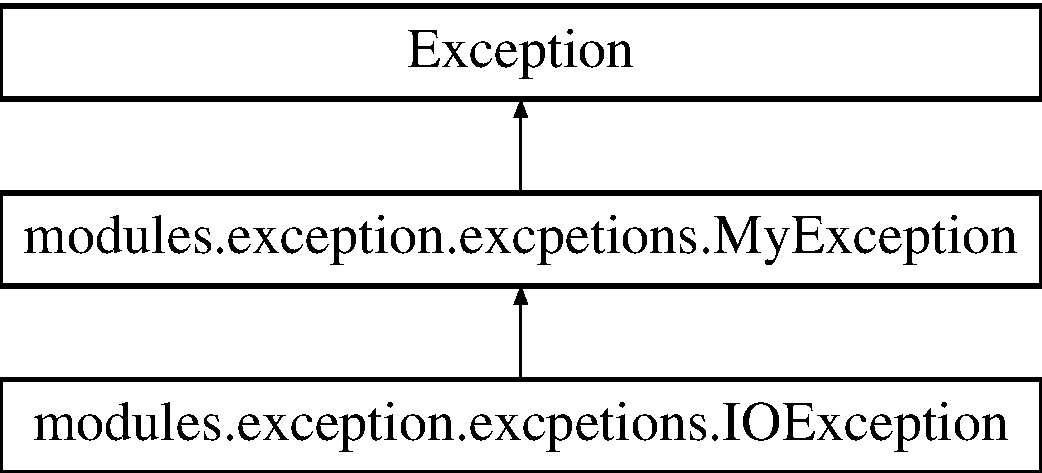
\includegraphics[height=3.000000cm]{classmodules_1_1exception_1_1excpetions_1_1_i_o_exception}
\end{center}
\end{figure}
\subsection*{Public Member Functions}
\begin{DoxyCompactItemize}
\item 
\mbox{\Hypertarget{classmodules_1_1exception_1_1excpetions_1_1_i_o_exception_a770b368ab4b21d16daff778631816de2}\label{classmodules_1_1exception_1_1excpetions_1_1_i_o_exception_a770b368ab4b21d16daff778631816de2}} 
def {\bfseries get\+\_\+type} (self)
\end{DoxyCompactItemize}


The documentation for this class was generated from the following file\+:\begin{DoxyCompactItemize}
\item 
exception/excpetions.\+py\end{DoxyCompactItemize}

\hypertarget{classmodules_1_1controller_1_1commands_1_1key_1_1_key}{}\section{modules.\+controller.\+commands.\+key.\+Key Class Reference}
\label{classmodules_1_1controller_1_1commands_1_1key_1_1_key}\index{modules.\+controller.\+commands.\+key.\+Key@{modules.\+controller.\+commands.\+key.\+Key}}
Inheritance diagram for modules.\+controller.\+commands.\+key.\+Key\+:\begin{figure}[H]
\begin{center}
\leavevmode
\includegraphics[height=2.000000cm]{classmodules_1_1controller_1_1commands_1_1key_1_1_key}
\end{center}
\end{figure}
\subsection*{Static Public Attributes}
\begin{DoxyCompactItemize}
\item 
\mbox{\Hypertarget{classmodules_1_1controller_1_1commands_1_1key_1_1_key_ab679820a2df346cd7cb493188e3b3fb5}\label{classmodules_1_1controller_1_1commands_1_1key_1_1_key_ab679820a2df346cd7cb493188e3b3fb5}} 
int {\bfseries Q\+U\+IT} = 0
\item 
\mbox{\Hypertarget{classmodules_1_1controller_1_1commands_1_1key_1_1_key_a49a8880acf6d2c9b0cb9d3c3cb64a142}\label{classmodules_1_1controller_1_1commands_1_1key_1_1_key_a49a8880acf6d2c9b0cb9d3c3cb64a142}} 
int {\bfseries A\+M\+O\+U\+NT} = 1
\item 
\mbox{\Hypertarget{classmodules_1_1controller_1_1commands_1_1key_1_1_key_a6e028b32c0b0b81fd497450190bb7c4f}\label{classmodules_1_1controller_1_1commands_1_1key_1_1_key_a6e028b32c0b0b81fd497450190bb7c4f}} 
int {\bfseries N\+A\+ME} = 2
\item 
\mbox{\Hypertarget{classmodules_1_1controller_1_1commands_1_1key_1_1_key_adad315b563f215b3b7456ea27e186133}\label{classmodules_1_1controller_1_1commands_1_1key_1_1_key_adad315b563f215b3b7456ea27e186133}} 
int {\bfseries D\+E\+N\+S\+I\+TY} = 3
\item 
\mbox{\Hypertarget{classmodules_1_1controller_1_1commands_1_1key_1_1_key_a6b94c7fcc0895e68908c2e0afe63965f}\label{classmodules_1_1controller_1_1commands_1_1key_1_1_key_a6b94c7fcc0895e68908c2e0afe63965f}} 
int {\bfseries S\+I\+ZE} = 4
\item 
\mbox{\Hypertarget{classmodules_1_1controller_1_1commands_1_1key_1_1_key_afba0308ded08dc0b66b1f3eda2118323}\label{classmodules_1_1controller_1_1commands_1_1key_1_1_key_afba0308ded08dc0b66b1f3eda2118323}} 
int {\bfseries P\+A\+TH} = 5
\item 
\mbox{\Hypertarget{classmodules_1_1controller_1_1commands_1_1key_1_1_key_af9fc685605638e0c35739d7a3a1ab5b3}\label{classmodules_1_1controller_1_1commands_1_1key_1_1_key_af9fc685605638e0c35739d7a3a1ab5b3}} 
int {\bfseries G\+E\+N\+E\+R\+A\+TE} = 6
\item 
\mbox{\Hypertarget{classmodules_1_1controller_1_1commands_1_1key_1_1_key_aac2aa6102323360c6b1dc7e276015da9}\label{classmodules_1_1controller_1_1commands_1_1key_1_1_key_aac2aa6102323360c6b1dc7e276015da9}} 
int {\bfseries S\+A\+V\+I\+N\+G\+\_\+\+P\+A\+TH} = 7
\item 
\mbox{\Hypertarget{classmodules_1_1controller_1_1commands_1_1key_1_1_key_a1d695ed554375bc23fd3c06295bd5158}\label{classmodules_1_1controller_1_1commands_1_1key_1_1_key_a1d695ed554375bc23fd3c06295bd5158}} 
int {\bfseries T\+R\+A\+IN} = 8
\item 
\mbox{\Hypertarget{classmodules_1_1controller_1_1commands_1_1key_1_1_key_a021f1becc3fdebde37afae78ab7fe4e1}\label{classmodules_1_1controller_1_1commands_1_1key_1_1_key_a021f1becc3fdebde37afae78ab7fe4e1}} 
int {\bfseries N\+E\+T\+W\+O\+RK} = 9
\item 
\mbox{\Hypertarget{classmodules_1_1controller_1_1commands_1_1key_1_1_key_a2e789e8e45efb4665b84ccf642447f76}\label{classmodules_1_1controller_1_1commands_1_1key_1_1_key_a2e789e8e45efb4665b84ccf642447f76}} 
int {\bfseries M\+O\+DE} = 10
\item 
\mbox{\Hypertarget{classmodules_1_1controller_1_1commands_1_1key_1_1_key_a73d5df57b028c18cdd0738664226cf82}\label{classmodules_1_1controller_1_1commands_1_1key_1_1_key_a73d5df57b028c18cdd0738664226cf82}} 
int {\bfseries S\+O\+L\+VE} = 11
\end{DoxyCompactItemize}


The documentation for this class was generated from the following file\+:\begin{DoxyCompactItemize}
\item 
controller/commands/key.\+py\end{DoxyCompactItemize}

\hypertarget{classmodules_1_1controller_1_1commands_1_1label__command_1_1_label_command}{}\section{modules.\+controller.\+commands.\+label\+\_\+command.\+Label\+Command Class Reference}
\label{classmodules_1_1controller_1_1commands_1_1label__command_1_1_label_command}\index{modules.\+controller.\+commands.\+label\+\_\+command.\+Label\+Command@{modules.\+controller.\+commands.\+label\+\_\+command.\+Label\+Command}}
Inheritance diagram for modules.\+controller.\+commands.\+label\+\_\+command.\+Label\+Command\+:\begin{figure}[H]
\begin{center}
\leavevmode
\includegraphics[height=2.000000cm]{classmodules_1_1controller_1_1commands_1_1label__command_1_1_label_command}
\end{center}
\end{figure}
\subsection*{Public Member Functions}
\begin{DoxyCompactItemize}
\item 
\mbox{\Hypertarget{classmodules_1_1controller_1_1commands_1_1label__command_1_1_label_command_ace24f8c42d67bc01da4f28eb10733c7f}\label{classmodules_1_1controller_1_1commands_1_1label__command_1_1_label_command_ace24f8c42d67bc01da4f28eb10733c7f}} 
def {\bfseries \+\_\+\+\_\+init\+\_\+\+\_\+} (self)
\item 
\mbox{\Hypertarget{classmodules_1_1controller_1_1commands_1_1label__command_1_1_label_command_a69a81d5739fcd1e4b188629b5beff8b1}\label{classmodules_1_1controller_1_1commands_1_1label__command_1_1_label_command_a69a81d5739fcd1e4b188629b5beff8b1}} 
def {\bfseries mode} (self)
\item 
\mbox{\Hypertarget{classmodules_1_1controller_1_1commands_1_1label__command_1_1_label_command_aae4e93651c3b4f8f743bd0d74a3a4995}\label{classmodules_1_1controller_1_1commands_1_1label__command_1_1_label_command_aae4e93651c3b4f8f743bd0d74a3a4995}} 
def {\bfseries config} (self)
\item 
\mbox{\Hypertarget{classmodules_1_1controller_1_1commands_1_1label__command_1_1_label_command_a68feb24f94df88021e3830d96ea4bb44}\label{classmodules_1_1controller_1_1commands_1_1label__command_1_1_label_command_a68feb24f94df88021e3830d96ea4bb44}} 
def {\bfseries execute} (self)
\item 
\mbox{\Hypertarget{classmodules_1_1controller_1_1commands_1_1label__command_1_1_label_command_a355cdbfdcd1ca33bb0640789d4dba1b7}\label{classmodules_1_1controller_1_1commands_1_1label__command_1_1_label_command_a355cdbfdcd1ca33bb0640789d4dba1b7}} 
def {\bfseries add\+\_\+args}
\end{DoxyCompactItemize}
\subsection*{Public Attributes}
\begin{DoxyCompactItemize}
\item 
\mbox{\Hypertarget{classmodules_1_1controller_1_1commands_1_1label__command_1_1_label_command_a822f83ec7884a77efee9fd3992259b69}\label{classmodules_1_1controller_1_1commands_1_1label__command_1_1_label_command_a822f83ec7884a77efee9fd3992259b69}} 
{\bfseries valid\+\_\+short\+\_\+arguments}
\item 
\mbox{\Hypertarget{classmodules_1_1controller_1_1commands_1_1label__command_1_1_label_command_a608a4e673b7e7d42d0c4909f2c6a3ed4}\label{classmodules_1_1controller_1_1commands_1_1label__command_1_1_label_command_a608a4e673b7e7d42d0c4909f2c6a3ed4}} 
{\bfseries valid\+\_\+long\+\_\+arguments}
\end{DoxyCompactItemize}


The documentation for this class was generated from the following file\+:\begin{DoxyCompactItemize}
\item 
controller/commands/label\+\_\+command.\+py\end{DoxyCompactItemize}

\hypertarget{classmodules_1_1model_1_1labeling__module_1_1labeling__module_1_1_labeling_module}{}\section{modules.\+model.\+labeling\+\_\+module.\+labeling\+\_\+module.\+Labeling\+Module Class Reference}
\label{classmodules_1_1model_1_1labeling__module_1_1labeling__module_1_1_labeling_module}\index{modules.\+model.\+labeling\+\_\+module.\+labeling\+\_\+module.\+Labeling\+Module@{modules.\+model.\+labeling\+\_\+module.\+labeling\+\_\+module.\+Labeling\+Module}}


This class handles the labeling of the matrices.  


\subsection*{Static Public Member Functions}
\begin{DoxyCompactItemize}
\item 
def \mbox{\hyperlink{classmodules_1_1model_1_1labeling__module_1_1labeling__module_1_1_labeling_module_ad62aae0768cc5dbab567c1764cd97402}{start}}
\begin{DoxyCompactList}\small\item\em Sets up the the class for the labeling process. \end{DoxyCompactList}\end{DoxyCompactItemize}


\subsection{Detailed Description}
This class handles the labeling of the matrices. 

\subsection{Member Function Documentation}
\mbox{\Hypertarget{classmodules_1_1model_1_1labeling__module_1_1labeling__module_1_1_labeling_module_ad62aae0768cc5dbab567c1764cd97402}\label{classmodules_1_1model_1_1labeling__module_1_1labeling__module_1_1_labeling_module_ad62aae0768cc5dbab567c1764cd97402}} 
\index{modules\+::model\+::labeling\+\_\+module\+::labeling\+\_\+module\+::\+Labeling\+Module@{modules\+::model\+::labeling\+\_\+module\+::labeling\+\_\+module\+::\+Labeling\+Module}!start@{start}}
\index{start@{start}!modules\+::model\+::labeling\+\_\+module\+::labeling\+\_\+module\+::\+Labeling\+Module@{modules\+::model\+::labeling\+\_\+module\+::labeling\+\_\+module\+::\+Labeling\+Module}}
\subsubsection{\texorpdfstring{start()}{start()}}
{\footnotesize\ttfamily def modules.\+model.\+labeling\+\_\+module.\+labeling\+\_\+module.\+Labeling\+Module.\+start (\begin{DoxyParamCaption}\item[{}]{path }\end{DoxyParamCaption})\hspace{0.3cm}{\ttfamily [static]}}



Sets up the the class for the labeling process. 


\begin{DoxyParams}{Parameters}
{\em path} & where the unlabeled matrices are located \\
\hline
{\em saving\+\_\+name} & name under which the labeled matrices will be saved \\
\hline
{\em saving\+\_\+path} & path to where the labeled matrices will be saved \\
\hline
\end{DoxyParams}


The documentation for this class was generated from the following file\+:\begin{DoxyCompactItemize}
\item 
model/labeling\+\_\+module/labeling\+\_\+module.\+py\end{DoxyCompactItemize}

\hypertarget{classmodules_1_1controller_1_1commands_1_1label__mode_1_1_label_mode}{}\section{modules.\+controller.\+commands.\+label\+\_\+mode.\+Label\+Mode Class Reference}
\label{classmodules_1_1controller_1_1commands_1_1label__mode_1_1_label_mode}\index{modules.\+controller.\+commands.\+label\+\_\+mode.\+Label\+Mode@{modules.\+controller.\+commands.\+label\+\_\+mode.\+Label\+Mode}}
Inheritance diagram for modules.\+controller.\+commands.\+label\+\_\+mode.\+Label\+Mode\+:\begin{figure}[H]
\begin{center}
\leavevmode
\includegraphics[height=2.000000cm]{classmodules_1_1controller_1_1commands_1_1label__mode_1_1_label_mode}
\end{center}
\end{figure}
\subsection*{Static Public Attributes}
\begin{DoxyCompactItemize}
\item 
\mbox{\Hypertarget{classmodules_1_1controller_1_1commands_1_1label__mode_1_1_label_mode_a3445fc4e2d7ec561611eb9e4471b3ffa}\label{classmodules_1_1controller_1_1commands_1_1label__mode_1_1_label_mode_a3445fc4e2d7ec561611eb9e4471b3ffa}} 
int {\bfseries L\+A\+B\+EL} = 1
\item 
\mbox{\Hypertarget{classmodules_1_1controller_1_1commands_1_1label__mode_1_1_label_mode_a46679913f9bddb670f0f2ae1b80254a0}\label{classmodules_1_1controller_1_1commands_1_1label__mode_1_1_label_mode_a46679913f9bddb670f0f2ae1b80254a0}} 
int {\bfseries A\+DD} = 2
\item 
\mbox{\Hypertarget{classmodules_1_1controller_1_1commands_1_1label__mode_1_1_label_mode_a8fa12d780974a25de1fe50231c56ec89}\label{classmodules_1_1controller_1_1commands_1_1label__mode_1_1_label_mode_a8fa12d780974a25de1fe50231c56ec89}} 
int {\bfseries R\+E\+M\+O\+VE} = 3
\end{DoxyCompactItemize}


The documentation for this class was generated from the following file\+:\begin{DoxyCompactItemize}
\item 
controller/commands/label\+\_\+mode.\+py\end{DoxyCompactItemize}

\hypertarget{classmodules_1_1shared_1_1loader_1_1_loader}{}\section{modules.\+shared.\+loader.\+Loader Class Reference}
\label{classmodules_1_1shared_1_1loader_1_1_loader}\index{modules.\+shared.\+loader.\+Loader@{modules.\+shared.\+loader.\+Loader}}


Class that handles the loading of matrices.  


\subsection*{Static Public Member Functions}
\begin{DoxyCompactItemize}
\item 
def \mbox{\hyperlink{classmodules_1_1shared_1_1loader_1_1_loader_a05b073bcb91c647ea4e6b47c71f40e94}{load}}
\begin{DoxyCompactList}\small\item\em Loads the dataset located at the input path. \end{DoxyCompactList}\end{DoxyCompactItemize}


\subsection{Detailed Description}
Class that handles the loading of matrices. 

\subsection{Member Function Documentation}
\mbox{\Hypertarget{classmodules_1_1shared_1_1loader_1_1_loader_a05b073bcb91c647ea4e6b47c71f40e94}\label{classmodules_1_1shared_1_1loader_1_1_loader_a05b073bcb91c647ea4e6b47c71f40e94}} 
\index{modules\+::shared\+::loader\+::\+Loader@{modules\+::shared\+::loader\+::\+Loader}!load@{load}}
\index{load@{load}!modules\+::shared\+::loader\+::\+Loader@{modules\+::shared\+::loader\+::\+Loader}}
\subsubsection{\texorpdfstring{load()}{load()}}
{\footnotesize\ttfamily def modules.\+shared.\+loader.\+Loader.\+load (\begin{DoxyParamCaption}\item[{}]{path }\end{DoxyParamCaption})\hspace{0.3cm}{\ttfamily [static]}}



Loads the dataset located at the input path. 


\begin{DoxyParams}{Parameters}
{\em path} & where the dataset is located \\
\hline
\end{DoxyParams}


The documentation for this class was generated from the following file\+:\begin{DoxyCompactItemize}
\item 
shared/loader.\+py\end{DoxyCompactItemize}

\hypertarget{classmodules_1_1shared_1_1matrix_1_1_matrix}{}\section{modules.\+shared.\+matrix.\+Matrix Class Reference}
\label{classmodules_1_1shared_1_1matrix_1_1_matrix}\index{modules.\+shared.\+matrix.\+Matrix@{modules.\+shared.\+matrix.\+Matrix}}


This class represents a matrix holding its values and size.  


\subsection*{Public Member Functions}
\begin{DoxyCompactItemize}
\item 
\mbox{\Hypertarget{classmodules_1_1shared_1_1matrix_1_1_matrix_a32926b695d2ea22c15fba2cd4aa6cfb6}\label{classmodules_1_1shared_1_1matrix_1_1_matrix_a32926b695d2ea22c15fba2cd4aa6cfb6}} 
def {\bfseries \+\_\+\+\_\+init\+\_\+\+\_\+}
\item 
\mbox{\Hypertarget{classmodules_1_1shared_1_1matrix_1_1_matrix_a703cf34dc79b4f0b94a8f8cf3fdf8b89}\label{classmodules_1_1shared_1_1matrix_1_1_matrix_a703cf34dc79b4f0b94a8f8cf3fdf8b89}} 
def {\bfseries values} (self)
\item 
\mbox{\Hypertarget{classmodules_1_1shared_1_1matrix_1_1_matrix_adca7e7e53fc7eaa5cb8d8273915ec4d6}\label{classmodules_1_1shared_1_1matrix_1_1_matrix_adca7e7e53fc7eaa5cb8d8273915ec4d6}} 
def {\bfseries size} (self)
\end{DoxyCompactItemize}


\subsection{Detailed Description}
This class represents a matrix holding its values and size. 

The documentation for this class was generated from the following file\+:\begin{DoxyCompactItemize}
\item 
shared/matrix.\+py\end{DoxyCompactItemize}

\hypertarget{classmodules_1_1exception_1_1excpetions_1_1_my_exception}{}\section{modules.\+exception.\+excpetions.\+My\+Exception Class Reference}
\label{classmodules_1_1exception_1_1excpetions_1_1_my_exception}\index{modules.\+exception.\+excpetions.\+My\+Exception@{modules.\+exception.\+excpetions.\+My\+Exception}}
Inheritance diagram for modules.\+exception.\+excpetions.\+My\+Exception\+:\begin{figure}[H]
\begin{center}
\leavevmode
\includegraphics[height=1.257485cm]{classmodules_1_1exception_1_1excpetions_1_1_my_exception}
\end{center}
\end{figure}
\subsection*{Public Member Functions}
\begin{DoxyCompactItemize}
\item 
\mbox{\Hypertarget{classmodules_1_1exception_1_1excpetions_1_1_my_exception_aa9a2bd83afa67e6b8515cb9a2f27d2e5}\label{classmodules_1_1exception_1_1excpetions_1_1_my_exception_aa9a2bd83afa67e6b8515cb9a2f27d2e5}} 
def {\bfseries \+\_\+\+\_\+init\+\_\+\+\_\+}
\item 
\mbox{\Hypertarget{classmodules_1_1exception_1_1excpetions_1_1_my_exception_a3f7ec639a138862780ee40c36206ea89}\label{classmodules_1_1exception_1_1excpetions_1_1_my_exception_a3f7ec639a138862780ee40c36206ea89}} 
def {\bfseries get\+\_\+info} (self)
\item 
\mbox{\Hypertarget{classmodules_1_1exception_1_1excpetions_1_1_my_exception_aa9751951fe01ee767067d74b3614c30c}\label{classmodules_1_1exception_1_1excpetions_1_1_my_exception_aa9751951fe01ee767067d74b3614c30c}} 
def {\bfseries get\+\_\+type} (self)
\end{DoxyCompactItemize}


The documentation for this class was generated from the following file\+:\begin{DoxyCompactItemize}
\item 
exception/excpetions.\+py\end{DoxyCompactItemize}

\hypertarget{classmodules_1_1view_1_1observable_1_1_observable}{}\section{modules.\+view.\+observable.\+Observable Class Reference}
\label{classmodules_1_1view_1_1observable_1_1_observable}\index{modules.\+view.\+observable.\+Observable@{modules.\+view.\+observable.\+Observable}}


Class for creating updating strings.  


\subsection*{Public Member Functions}
\begin{DoxyCompactItemize}
\item 
\mbox{\Hypertarget{classmodules_1_1view_1_1observable_1_1_observable_ad15fa226b4f9a978fc0e105d6a06b181}\label{classmodules_1_1view_1_1observable_1_1_observable_ad15fa226b4f9a978fc0e105d6a06b181}} 
def {\bfseries \+\_\+\+\_\+init\+\_\+\+\_\+} (self)
\item 
def \mbox{\hyperlink{classmodules_1_1view_1_1observable_1_1_observable_a148631fbe8f3f1cf66dff03322a48882}{next}}
\begin{DoxyCompactList}\small\item\em Method to trigger an update on all subscribers. \end{DoxyCompactList}\item 
def \mbox{\hyperlink{classmodules_1_1view_1_1observable_1_1_observable_a1560584bfd33f7aac04c288723785264}{add\+\_\+subscriber}}
\begin{DoxyCompactList}\small\item\em A subscriber can be added with this function. \end{DoxyCompactList}\item 
def \mbox{\hyperlink{classmodules_1_1view_1_1observable_1_1_observable_a1545faf481765b0a7a7dd17b3e7c9c35}{remove\+\_\+subscriber}}
\begin{DoxyCompactList}\small\item\em A subscriber can be removed with this function. \end{DoxyCompactList}\end{DoxyCompactItemize}


\subsection{Detailed Description}
Class for creating updating strings. 

Can be used if you want to create an string in the view, that will be updated with new values 

\subsection{Member Function Documentation}
\mbox{\Hypertarget{classmodules_1_1view_1_1observable_1_1_observable_a1560584bfd33f7aac04c288723785264}\label{classmodules_1_1view_1_1observable_1_1_observable_a1560584bfd33f7aac04c288723785264}} 
\index{modules\+::view\+::observable\+::\+Observable@{modules\+::view\+::observable\+::\+Observable}!add\+\_\+subscriber@{add\+\_\+subscriber}}
\index{add\+\_\+subscriber@{add\+\_\+subscriber}!modules\+::view\+::observable\+::\+Observable@{modules\+::view\+::observable\+::\+Observable}}
\subsubsection{\texorpdfstring{add\+\_\+subscriber()}{add\_subscriber()}}
{\footnotesize\ttfamily def modules.\+view.\+observable.\+Observable.\+add\+\_\+subscriber (\begin{DoxyParamCaption}\item[{}]{self,  }\item[{}]{subscriber }\end{DoxyParamCaption})}



A subscriber can be added with this function. 


\begin{DoxyParams}{Parameters}
{\em subscriber} & the subscriber that wants to receive status updates \\
\hline
\end{DoxyParams}
\mbox{\Hypertarget{classmodules_1_1view_1_1observable_1_1_observable_a148631fbe8f3f1cf66dff03322a48882}\label{classmodules_1_1view_1_1observable_1_1_observable_a148631fbe8f3f1cf66dff03322a48882}} 
\index{modules\+::view\+::observable\+::\+Observable@{modules\+::view\+::observable\+::\+Observable}!next@{next}}
\index{next@{next}!modules\+::view\+::observable\+::\+Observable@{modules\+::view\+::observable\+::\+Observable}}
\subsubsection{\texorpdfstring{next()}{next()}}
{\footnotesize\ttfamily def modules.\+view.\+observable.\+Observable.\+next (\begin{DoxyParamCaption}\item[{}]{self,  }\item[{}]{update }\end{DoxyParamCaption})}



Method to trigger an update on all subscribers. 


\begin{DoxyParams}{Parameters}
{\em update} & the new value \\
\hline
\end{DoxyParams}
\mbox{\Hypertarget{classmodules_1_1view_1_1observable_1_1_observable_a1545faf481765b0a7a7dd17b3e7c9c35}\label{classmodules_1_1view_1_1observable_1_1_observable_a1545faf481765b0a7a7dd17b3e7c9c35}} 
\index{modules\+::view\+::observable\+::\+Observable@{modules\+::view\+::observable\+::\+Observable}!remove\+\_\+subscriber@{remove\+\_\+subscriber}}
\index{remove\+\_\+subscriber@{remove\+\_\+subscriber}!modules\+::view\+::observable\+::\+Observable@{modules\+::view\+::observable\+::\+Observable}}
\subsubsection{\texorpdfstring{remove\+\_\+subscriber()}{remove\_subscriber()}}
{\footnotesize\ttfamily def modules.\+view.\+observable.\+Observable.\+remove\+\_\+subscriber (\begin{DoxyParamCaption}\item[{}]{self,  }\item[{}]{subscriber }\end{DoxyParamCaption})}



A subscriber can be removed with this function. 


\begin{DoxyParams}{Parameters}
{\em subscriber} & the subscriber who wants to be removed from receiving status updates \\
\hline
\end{DoxyParams}


The documentation for this class was generated from the following file\+:\begin{DoxyCompactItemize}
\item 
view/observable.\+py\end{DoxyCompactItemize}

\hypertarget{classmodules_1_1view_1_1output__service_1_1_output_service}{}\section{modules.\+view.\+output\+\_\+service.\+Output\+Service Class Reference}
\label{classmodules_1_1view_1_1output__service_1_1_output_service}\index{modules.\+view.\+output\+\_\+service.\+Output\+Service@{modules.\+view.\+output\+\_\+service.\+Output\+Service}}


Interface for services that can be registered to a module.  


Inheritance diagram for modules.\+view.\+output\+\_\+service.\+Output\+Service\+:\begin{figure}[H]
\begin{center}
\leavevmode
\includegraphics[height=2.000000cm]{classmodules_1_1view_1_1output__service_1_1_output_service}
\end{center}
\end{figure}
\subsection*{Public Member Functions}
\begin{DoxyCompactItemize}
\item 
def \mbox{\hyperlink{classmodules_1_1view_1_1output__service_1_1_output_service_a8304983652bdd3c49eb620b7e20b4c20}{print\+\_\+line}}
\begin{DoxyCompactList}\small\item\em Prints a line to the view. \end{DoxyCompactList}\item 
def \mbox{\hyperlink{classmodules_1_1view_1_1output__service_1_1_output_service_aa5179629e76d57412ac243947a252331}{print\+\_\+stream}}
\begin{DoxyCompactList}\small\item\em Prints an self overriding string. \end{DoxyCompactList}\item 
def \mbox{\hyperlink{classmodules_1_1view_1_1output__service_1_1_output_service_a1cc2f7091e8bd0aac36200ebccf90e25}{print\+\_\+error}}
\begin{DoxyCompactList}\small\item\em Prints an exception to the view. \end{DoxyCompactList}\item 
def \mbox{\hyperlink{classmodules_1_1view_1_1output__service_1_1_output_service_ae50d47ab13cb38996d179c75bd2ee58e}{print\+\_\+matrix}}
\begin{DoxyCompactList}\small\item\em Prints a matrix to the view. \end{DoxyCompactList}\end{DoxyCompactItemize}


\subsection{Detailed Description}
Interface for services that can be registered to a module. 

\subsection{Member Function Documentation}
\mbox{\Hypertarget{classmodules_1_1view_1_1output__service_1_1_output_service_a1cc2f7091e8bd0aac36200ebccf90e25}\label{classmodules_1_1view_1_1output__service_1_1_output_service_a1cc2f7091e8bd0aac36200ebccf90e25}} 
\index{modules\+::view\+::output\+\_\+service\+::\+Output\+Service@{modules\+::view\+::output\+\_\+service\+::\+Output\+Service}!print\+\_\+error@{print\+\_\+error}}
\index{print\+\_\+error@{print\+\_\+error}!modules\+::view\+::output\+\_\+service\+::\+Output\+Service@{modules\+::view\+::output\+\_\+service\+::\+Output\+Service}}
\subsubsection{\texorpdfstring{print\+\_\+error()}{print\_error()}}
{\footnotesize\ttfamily def modules.\+view.\+output\+\_\+service.\+Output\+Service.\+print\+\_\+error (\begin{DoxyParamCaption}\item[{}]{self,  }\item[{}]{error }\end{DoxyParamCaption})}



Prints an exception to the view. 


\begin{DoxyParams}{Parameters}
{\em exception} & the error holding a message \\
\hline
\end{DoxyParams}
\mbox{\Hypertarget{classmodules_1_1view_1_1output__service_1_1_output_service_a8304983652bdd3c49eb620b7e20b4c20}\label{classmodules_1_1view_1_1output__service_1_1_output_service_a8304983652bdd3c49eb620b7e20b4c20}} 
\index{modules\+::view\+::output\+\_\+service\+::\+Output\+Service@{modules\+::view\+::output\+\_\+service\+::\+Output\+Service}!print\+\_\+line@{print\+\_\+line}}
\index{print\+\_\+line@{print\+\_\+line}!modules\+::view\+::output\+\_\+service\+::\+Output\+Service@{modules\+::view\+::output\+\_\+service\+::\+Output\+Service}}
\subsubsection{\texorpdfstring{print\+\_\+line()}{print\_line()}}
{\footnotesize\ttfamily def modules.\+view.\+output\+\_\+service.\+Output\+Service.\+print\+\_\+line (\begin{DoxyParamCaption}\item[{}]{self,  }\item[{}]{line }\end{DoxyParamCaption})}



Prints a line to the view. 


\begin{DoxyParams}{Parameters}
{\em line} & the line that should be printed \\
\hline
\end{DoxyParams}
\mbox{\Hypertarget{classmodules_1_1view_1_1output__service_1_1_output_service_ae50d47ab13cb38996d179c75bd2ee58e}\label{classmodules_1_1view_1_1output__service_1_1_output_service_ae50d47ab13cb38996d179c75bd2ee58e}} 
\index{modules\+::view\+::output\+\_\+service\+::\+Output\+Service@{modules\+::view\+::output\+\_\+service\+::\+Output\+Service}!print\+\_\+matrix@{print\+\_\+matrix}}
\index{print\+\_\+matrix@{print\+\_\+matrix}!modules\+::view\+::output\+\_\+service\+::\+Output\+Service@{modules\+::view\+::output\+\_\+service\+::\+Output\+Service}}
\subsubsection{\texorpdfstring{print\+\_\+matrix()}{print\_matrix()}}
{\footnotesize\ttfamily def modules.\+view.\+output\+\_\+service.\+Output\+Service.\+print\+\_\+matrix (\begin{DoxyParamCaption}\item[{}]{self,  }\item[{}]{matrix }\end{DoxyParamCaption})}



Prints a matrix to the view. 


\begin{DoxyParams}{Parameters}
{\em matrix} & the matrix that will be displayed \\
\hline
\end{DoxyParams}
\mbox{\Hypertarget{classmodules_1_1view_1_1output__service_1_1_output_service_aa5179629e76d57412ac243947a252331}\label{classmodules_1_1view_1_1output__service_1_1_output_service_aa5179629e76d57412ac243947a252331}} 
\index{modules\+::view\+::output\+\_\+service\+::\+Output\+Service@{modules\+::view\+::output\+\_\+service\+::\+Output\+Service}!print\+\_\+stream@{print\+\_\+stream}}
\index{print\+\_\+stream@{print\+\_\+stream}!modules\+::view\+::output\+\_\+service\+::\+Output\+Service@{modules\+::view\+::output\+\_\+service\+::\+Output\+Service}}
\subsubsection{\texorpdfstring{print\+\_\+stream()}{print\_stream()}}
{\footnotesize\ttfamily def modules.\+view.\+output\+\_\+service.\+Output\+Service.\+print\+\_\+stream (\begin{DoxyParamCaption}\item[{}]{self,  }\item[{}]{message }\end{DoxyParamCaption})}



Prints an self overriding string. 


\begin{DoxyParams}{Parameters}
{\em message} & the line that will stay the same \\
\hline
{\em observable} & where the updates of the values can be retrieved \\
\hline
\end{DoxyParams}


The documentation for this class was generated from the following file\+:\begin{DoxyCompactItemize}
\item 
view/output\+\_\+service.\+py\end{DoxyCompactItemize}

\hypertarget{classmodules_1_1model_1_1labeling__module_1_1preconditioner_1_1_preconditioner}{}\section{modules.\+model.\+labeling\+\_\+module.\+preconditioner.\+Preconditioner Class Reference}
\label{classmodules_1_1model_1_1labeling__module_1_1preconditioner_1_1_preconditioner}\index{modules.\+model.\+labeling\+\_\+module.\+preconditioner.\+Preconditioner@{modules.\+model.\+labeling\+\_\+module.\+preconditioner.\+Preconditioner}}


Abstract class that represents the preconditioners which can be applied to a matrix to fasten the solving process.  


\subsection*{Public Member Functions}
\begin{DoxyCompactItemize}
\item 
def \mbox{\hyperlink{classmodules_1_1model_1_1labeling__module_1_1preconditioner_1_1_preconditioner_a55fddb23099daf1c639c7d2612b146f9}{get\+\_\+preconditioner}} (self)
\begin{DoxyCompactList}\small\item\em Get the name of the preconditioner that will be understood by the ginkgo library. \end{DoxyCompactList}\end{DoxyCompactItemize}


\subsection{Detailed Description}
Abstract class that represents the preconditioners which can be applied to a matrix to fasten the solving process. 

\subsection{Member Function Documentation}
\mbox{\Hypertarget{classmodules_1_1model_1_1labeling__module_1_1preconditioner_1_1_preconditioner_a55fddb23099daf1c639c7d2612b146f9}\label{classmodules_1_1model_1_1labeling__module_1_1preconditioner_1_1_preconditioner_a55fddb23099daf1c639c7d2612b146f9}} 
\index{modules\+::model\+::labeling\+\_\+module\+::preconditioner\+::\+Preconditioner@{modules\+::model\+::labeling\+\_\+module\+::preconditioner\+::\+Preconditioner}!get\+\_\+preconditioner@{get\+\_\+preconditioner}}
\index{get\+\_\+preconditioner@{get\+\_\+preconditioner}!modules\+::model\+::labeling\+\_\+module\+::preconditioner\+::\+Preconditioner@{modules\+::model\+::labeling\+\_\+module\+::preconditioner\+::\+Preconditioner}}
\subsubsection{\texorpdfstring{get\+\_\+preconditioner()}{get\_preconditioner()}}
{\footnotesize\ttfamily def modules.\+model.\+labeling\+\_\+module.\+preconditioner.\+Preconditioner.\+get\+\_\+preconditioner (\begin{DoxyParamCaption}\item[{}]{self,  }\item[{}]{str }\end{DoxyParamCaption})}



Get the name of the preconditioner that will be understood by the ginkgo library. 

\begin{DoxyReturn}{Returns}
name of the preconditioner that can be used in ginkgo 
\end{DoxyReturn}


The documentation for this class was generated from the following file\+:\begin{DoxyCompactItemize}
\item 
model/labeling\+\_\+module/preconditioner.\+py\end{DoxyCompactItemize}

\hypertarget{classmodules_1_1controller_1_1commands_1_1quit__command_1_1_quit_command}{}\section{modules.\+controller.\+commands.\+quit\+\_\+command.\+Quit\+Command Class Reference}
\label{classmodules_1_1controller_1_1commands_1_1quit__command_1_1_quit_command}\index{modules.\+controller.\+commands.\+quit\+\_\+command.\+Quit\+Command@{modules.\+controller.\+commands.\+quit\+\_\+command.\+Quit\+Command}}
Inheritance diagram for modules.\+controller.\+commands.\+quit\+\_\+command.\+Quit\+Command\+:\begin{figure}[H]
\begin{center}
\leavevmode
\includegraphics[height=2.000000cm]{classmodules_1_1controller_1_1commands_1_1quit__command_1_1_quit_command}
\end{center}
\end{figure}
\subsection*{Public Member Functions}
\begin{DoxyCompactItemize}
\item 
\mbox{\Hypertarget{classmodules_1_1controller_1_1commands_1_1quit__command_1_1_quit_command_a6eb669d9493b50e50f09027fe6d06f4c}\label{classmodules_1_1controller_1_1commands_1_1quit__command_1_1_quit_command_a6eb669d9493b50e50f09027fe6d06f4c}} 
def {\bfseries execute} (self)
\end{DoxyCompactItemize}


The documentation for this class was generated from the following file\+:\begin{DoxyCompactItemize}
\item 
controller/commands/quit\+\_\+command.\+py\end{DoxyCompactItemize}

\hypertarget{classmodules_1_1shared_1_1saver_1_1_saver}{}\section{modules.\+shared.\+saver.\+Saver Class Reference}
\label{classmodules_1_1shared_1_1saver_1_1_saver}\index{modules.\+shared.\+saver.\+Saver@{modules.\+shared.\+saver.\+Saver}}


Class that handles the saving of datasets.  


\subsection*{Static Public Member Functions}
\begin{DoxyCompactItemize}
\item 
def \mbox{\hyperlink{classmodules_1_1shared_1_1saver_1_1_saver_a56bd2d277b7f1184d3436738e8aff510}{save}}
\begin{DoxyCompactList}\small\item\em This method saves a dataset to a specified location. \end{DoxyCompactList}\end{DoxyCompactItemize}


\subsection{Detailed Description}
Class that handles the saving of datasets. 

\subsection{Member Function Documentation}
\mbox{\Hypertarget{classmodules_1_1shared_1_1saver_1_1_saver_a56bd2d277b7f1184d3436738e8aff510}\label{classmodules_1_1shared_1_1saver_1_1_saver_a56bd2d277b7f1184d3436738e8aff510}} 
\index{modules\+::shared\+::saver\+::\+Saver@{modules\+::shared\+::saver\+::\+Saver}!save@{save}}
\index{save@{save}!modules\+::shared\+::saver\+::\+Saver@{modules\+::shared\+::saver\+::\+Saver}}
\subsubsection{\texorpdfstring{save()}{save()}}
{\footnotesize\ttfamily def modules.\+shared.\+saver.\+Saver.\+save (\begin{DoxyParamCaption}\item[{}]{dataset,  }\item[{}]{name }\end{DoxyParamCaption})\hspace{0.3cm}{\ttfamily [static]}}



This method saves a dataset to a specified location. 


\begin{DoxyParams}{Parameters}
{\em dataset} & that will be saved \\
\hline
{\em name} & under which it will be saved \\
\hline
{\em path} & where it will be saved \\
\hline
\end{DoxyParams}


The documentation for this class was generated from the following file\+:\begin{DoxyCompactItemize}
\item 
shared/saver.\+py\end{DoxyCompactItemize}

\hypertarget{classmodules_1_1model_1_1labeling__module_1_1solver_1_1_solver}{}\section{modules.\+model.\+labeling\+\_\+module.\+solver.\+Solver Class Reference}
\label{classmodules_1_1model_1_1labeling__module_1_1solver_1_1_solver}\index{modules.\+model.\+labeling\+\_\+module.\+solver.\+Solver@{modules.\+model.\+labeling\+\_\+module.\+solver.\+Solver}}


Abstract class representing the various solvers tht can be executed on the matrices.  


\subsection*{Public Member Functions}
\begin{DoxyCompactItemize}
\item 
def \mbox{\hyperlink{classmodules_1_1model_1_1labeling__module_1_1solver_1_1_solver_a8e681ff0a63b2b324a0dfdec17efcaf7}{execute}}
\begin{DoxyCompactList}\small\item\em starts the solving of a matrix \end{DoxyCompactList}\end{DoxyCompactItemize}


\subsection{Detailed Description}
Abstract class representing the various solvers tht can be executed on the matrices. 

\subsection{Member Function Documentation}
\mbox{\Hypertarget{classmodules_1_1model_1_1labeling__module_1_1solver_1_1_solver_a8e681ff0a63b2b324a0dfdec17efcaf7}\label{classmodules_1_1model_1_1labeling__module_1_1solver_1_1_solver_a8e681ff0a63b2b324a0dfdec17efcaf7}} 
\index{modules\+::model\+::labeling\+\_\+module\+::solver\+::\+Solver@{modules\+::model\+::labeling\+\_\+module\+::solver\+::\+Solver}!execute@{execute}}
\index{execute@{execute}!modules\+::model\+::labeling\+\_\+module\+::solver\+::\+Solver@{modules\+::model\+::labeling\+\_\+module\+::solver\+::\+Solver}}
\subsubsection{\texorpdfstring{execute()}{execute()}}
{\footnotesize\ttfamily def modules.\+model.\+labeling\+\_\+module.\+solver.\+Solver.\+execute (\begin{DoxyParamCaption}\item[{}]{self,  }\item[{}]{matrix }\end{DoxyParamCaption})}



starts the solving of a matrix 


\begin{DoxyParams}{Parameters}
{\em matrix} & which will be solved \\
\hline
{\em preconditioner} & which will be applied on the matrix to fasten the solving process \\
\hline
\end{DoxyParams}


The documentation for this class was generated from the following file\+:\begin{DoxyCompactItemize}
\item 
model/labeling\+\_\+module/solver.\+py\end{DoxyCompactItemize}

\hypertarget{classmodules_1_1model_1_1collector__module_1_1ssget_1_1_s_s_get}{}\section{modules.\+model.\+collector\+\_\+module.\+ssget.\+S\+S\+Get Class Reference}
\label{classmodules_1_1model_1_1collector__module_1_1ssget_1_1_s_s_get}\index{modules.\+model.\+collector\+\_\+module.\+ssget.\+S\+S\+Get@{modules.\+model.\+collector\+\_\+module.\+ssget.\+S\+S\+Get}}


This class handles the communication with the suit sparse matrix collection using the ssget tool.  


\subsection*{Static Public Member Functions}
\begin{DoxyCompactItemize}
\item 
def \mbox{\hyperlink{classmodules_1_1model_1_1collector__module_1_1ssget_1_1_s_s_get_af928bff258646991311a9d68b83e8c10}{get\+\_\+matrix}}
\begin{DoxyCompactList}\small\item\em Gets you a matrix. \end{DoxyCompactList}\end{DoxyCompactItemize}


\subsection{Detailed Description}
This class handles the communication with the suit sparse matrix collection using the ssget tool. 

\subsection{Member Function Documentation}
\mbox{\Hypertarget{classmodules_1_1model_1_1collector__module_1_1ssget_1_1_s_s_get_af928bff258646991311a9d68b83e8c10}\label{classmodules_1_1model_1_1collector__module_1_1ssget_1_1_s_s_get_af928bff258646991311a9d68b83e8c10}} 
\index{modules\+::model\+::collector\+\_\+module\+::ssget\+::\+S\+S\+Get@{modules\+::model\+::collector\+\_\+module\+::ssget\+::\+S\+S\+Get}!get\+\_\+matrix@{get\+\_\+matrix}}
\index{get\+\_\+matrix@{get\+\_\+matrix}!modules\+::model\+::collector\+\_\+module\+::ssget\+::\+S\+S\+Get@{modules\+::model\+::collector\+\_\+module\+::ssget\+::\+S\+S\+Get}}
\subsubsection{\texorpdfstring{get\+\_\+matrix()}{get\_matrix()}}
{\footnotesize\ttfamily def modules.\+model.\+collector\+\_\+module.\+ssget.\+S\+S\+Get.\+get\+\_\+matrix (\begin{DoxyParamCaption}\item[{}]{size }\end{DoxyParamCaption})\hspace{0.3cm}{\ttfamily [static]}}



Gets you a matrix. 

\begin{DoxyReturn}{Returns}
matrix that has been downloaded 
\end{DoxyReturn}


The documentation for this class was generated from the following file\+:\begin{DoxyCompactItemize}
\item 
model/collector\+\_\+module/ssget.\+py\end{DoxyCompactItemize}

\hypertarget{classmodules_1_1view_1_1subscriber_1_1_subscriber}{}\section{modules.\+view.\+subscriber.\+Subscriber Class Reference}
\label{classmodules_1_1view_1_1subscriber_1_1_subscriber}\index{modules.\+view.\+subscriber.\+Subscriber@{modules.\+view.\+subscriber.\+Subscriber}}


Class than can be registered to an observable.  


Inheritance diagram for modules.\+view.\+subscriber.\+Subscriber\+:\begin{figure}[H]
\begin{center}
\leavevmode
\includegraphics[height=2.000000cm]{classmodules_1_1view_1_1subscriber_1_1_subscriber}
\end{center}
\end{figure}
\subsection*{Public Member Functions}
\begin{DoxyCompactItemize}
\item 
def \mbox{\hyperlink{classmodules_1_1view_1_1subscriber_1_1_subscriber_a270f8cd70bacb880fa467ee870c2d959}{update}}
\begin{DoxyCompactList}\small\item\em will be triggered when new values arrive \end{DoxyCompactList}\end{DoxyCompactItemize}


\subsection{Detailed Description}
Class than can be registered to an observable. 

\subsection{Member Function Documentation}
\mbox{\Hypertarget{classmodules_1_1view_1_1subscriber_1_1_subscriber_a270f8cd70bacb880fa467ee870c2d959}\label{classmodules_1_1view_1_1subscriber_1_1_subscriber_a270f8cd70bacb880fa467ee870c2d959}} 
\index{modules\+::view\+::subscriber\+::\+Subscriber@{modules\+::view\+::subscriber\+::\+Subscriber}!update@{update}}
\index{update@{update}!modules\+::view\+::subscriber\+::\+Subscriber@{modules\+::view\+::subscriber\+::\+Subscriber}}
\subsubsection{\texorpdfstring{update()}{update()}}
{\footnotesize\ttfamily def modules.\+view.\+subscriber.\+Subscriber.\+update (\begin{DoxyParamCaption}\item[{}]{self,  }\item[{}]{value }\end{DoxyParamCaption})}



will be triggered when new values arrive 


\begin{DoxyParams}{Parameters}
{\em value} & the new value that was passed to the observable \\
\hline
\end{DoxyParams}


The documentation for this class was generated from the following file\+:\begin{DoxyCompactItemize}
\item 
view/subscriber.\+py\end{DoxyCompactItemize}

\hypertarget{classmodules_1_1controller_1_1commands_1_1train__command_1_1_train_command}{}\section{modules.\+controller.\+commands.\+train\+\_\+command.\+Train\+Command Class Reference}
\label{classmodules_1_1controller_1_1commands_1_1train__command_1_1_train_command}\index{modules.\+controller.\+commands.\+train\+\_\+command.\+Train\+Command@{modules.\+controller.\+commands.\+train\+\_\+command.\+Train\+Command}}
Inheritance diagram for modules.\+controller.\+commands.\+train\+\_\+command.\+Train\+Command\+:\begin{figure}[H]
\begin{center}
\leavevmode
\includegraphics[height=2.000000cm]{classmodules_1_1controller_1_1commands_1_1train__command_1_1_train_command}
\end{center}
\end{figure}
\subsection*{Public Member Functions}
\begin{DoxyCompactItemize}
\item 
\mbox{\Hypertarget{classmodules_1_1controller_1_1commands_1_1train__command_1_1_train_command_a0f1babed0387698beca400b8add14688}\label{classmodules_1_1controller_1_1commands_1_1train__command_1_1_train_command_a0f1babed0387698beca400b8add14688}} 
def {\bfseries \+\_\+\+\_\+init\+\_\+\+\_\+} (self)
\item 
\mbox{\Hypertarget{classmodules_1_1controller_1_1commands_1_1train__command_1_1_train_command_a5a8a02925c5627c5c6438dd5a2dfd27f}\label{classmodules_1_1controller_1_1commands_1_1train__command_1_1_train_command_a5a8a02925c5627c5c6438dd5a2dfd27f}} 
def {\bfseries execute} (self)
\end{DoxyCompactItemize}
\subsection*{Public Attributes}
\begin{DoxyCompactItemize}
\item 
\mbox{\Hypertarget{classmodules_1_1controller_1_1commands_1_1train__command_1_1_train_command_aa041e94abaf0fc9318d7d1957205a43f}\label{classmodules_1_1controller_1_1commands_1_1train__command_1_1_train_command_aa041e94abaf0fc9318d7d1957205a43f}} 
{\bfseries valid\+\_\+short\+\_\+arguments}
\item 
\mbox{\Hypertarget{classmodules_1_1controller_1_1commands_1_1train__command_1_1_train_command_a4f6da9d06babc3bcc769f83eceb35c4c}\label{classmodules_1_1controller_1_1commands_1_1train__command_1_1_train_command_a4f6da9d06babc3bcc769f83eceb35c4c}} 
{\bfseries valid\+\_\+long\+\_\+arguments}
\end{DoxyCompactItemize}


The documentation for this class was generated from the following file\+:\begin{DoxyCompactItemize}
\item 
controller/commands/train\+\_\+command.\+py\end{DoxyCompactItemize}

\hypertarget{classmodules_1_1model_1_1training__module_1_1training__module_1_1_training_module}{}\section{modules.\+model.\+training\+\_\+module.\+training\+\_\+module.\+Training\+Module Class Reference}
\label{classmodules_1_1model_1_1training__module_1_1training__module_1_1_training_module}\index{modules.\+model.\+training\+\_\+module.\+training\+\_\+module.\+Training\+Module@{modules.\+model.\+training\+\_\+module.\+training\+\_\+module.\+Training\+Module}}


This class handles the training of the neural network.  


\subsection*{Static Public Member Functions}
\begin{DoxyCompactItemize}
\item 
def \mbox{\hyperlink{classmodules_1_1model_1_1training__module_1_1training__module_1_1_training_module_a0e906a21edf9cedca9a8d21743fe937b}{train}}
\begin{DoxyCompactList}\small\item\em trains the neural network labeled matrices \end{DoxyCompactList}\end{DoxyCompactItemize}


\subsection{Detailed Description}
This class handles the training of the neural network. 

\subsection{Member Function Documentation}
\mbox{\Hypertarget{classmodules_1_1model_1_1training__module_1_1training__module_1_1_training_module_a0e906a21edf9cedca9a8d21743fe937b}\label{classmodules_1_1model_1_1training__module_1_1training__module_1_1_training_module_a0e906a21edf9cedca9a8d21743fe937b}} 
\index{modules\+::model\+::training\+\_\+module\+::training\+\_\+module\+::\+Training\+Module@{modules\+::model\+::training\+\_\+module\+::training\+\_\+module\+::\+Training\+Module}!train@{train}}
\index{train@{train}!modules\+::model\+::training\+\_\+module\+::training\+\_\+module\+::\+Training\+Module@{modules\+::model\+::training\+\_\+module\+::training\+\_\+module\+::\+Training\+Module}}
\subsubsection{\texorpdfstring{train()}{train()}}
{\footnotesize\ttfamily def modules.\+model.\+training\+\_\+module.\+training\+\_\+module.\+Training\+Module.\+train (\begin{DoxyParamCaption}\item[{}]{matrices\+\_\+path }\end{DoxyParamCaption})\hspace{0.3cm}{\ttfamily [static]}}



trains the neural network labeled matrices 


\begin{DoxyParams}{Parameters}
{\em matrices\+\_\+path} & path where the labeled matrices are located \\
\hline
{\em neural\+\_\+network\+\_\+path} & path where are existing neural network is located if you want to improve one \\
\hline
{\em name} & under which the trained network will be saved \\
\hline
{\em saving\+\_\+path} & path to where the trained network will be saved \\
\hline
\end{DoxyParams}


The documentation for this class was generated from the following file\+:\begin{DoxyCompactItemize}
\item 
model/training\+\_\+module/training\+\_\+module.\+py\end{DoxyCompactItemize}

\hypertarget{classmodules_1_1shared_1_1validator_1_1_validator}{}\section{modules.\+shared.\+validator.\+Validator Class Reference}
\label{classmodules_1_1shared_1_1validator_1_1_validator}\index{modules.\+shared.\+validator.\+Validator@{modules.\+shared.\+validator.\+Validator}}
\subsection*{Static Public Member Functions}
\begin{DoxyCompactItemize}
\item 
def \mbox{\hyperlink{classmodules_1_1shared_1_1validator_1_1_validator_a5c2053342eeeffe53605742687e40b53}{validate}}
\begin{DoxyCompactList}\small\item\em This function checks if a given matrix can be used by our program. \end{DoxyCompactList}\end{DoxyCompactItemize}


\subsection{Member Function Documentation}
\mbox{\Hypertarget{classmodules_1_1shared_1_1validator_1_1_validator_a5c2053342eeeffe53605742687e40b53}\label{classmodules_1_1shared_1_1validator_1_1_validator_a5c2053342eeeffe53605742687e40b53}} 
\index{modules\+::shared\+::validator\+::\+Validator@{modules\+::shared\+::validator\+::\+Validator}!validate@{validate}}
\index{validate@{validate}!modules\+::shared\+::validator\+::\+Validator@{modules\+::shared\+::validator\+::\+Validator}}
\subsubsection{\texorpdfstring{validate()}{validate()}}
{\footnotesize\ttfamily def modules.\+shared.\+validator.\+Validator.\+validate (\begin{DoxyParamCaption}\item[{}]{matrix }\end{DoxyParamCaption})\hspace{0.3cm}{\ttfamily [static]}}



This function checks if a given matrix can be used by our program. 


\begin{DoxyParams}{Parameters}
{\em matrix} & which will be checked \\
\hline
\end{DoxyParams}


The documentation for this class was generated from the following file\+:\begin{DoxyCompactItemize}
\item 
shared/validator.\+py\end{DoxyCompactItemize}

%--- End generated contents ---

% Index
\backmatter
\newpage
\phantomsection
\clearemptydoublepage
\addcontentsline{toc}{chapter}{Index}
\printindex

\end{document}
